% I use VSCode with LaTex Workshop which shows PDF preview at the right side. There are some other UIs
% TextWorkshop on Windows, TexMaker on Mac. But I use VSCode.
% To generate PDF: pdflatext user_guide.tex
% Copyright (c) Spenego Software LLC

% This is a LaTex document. We are using LaTex because writing documents should be fun.
%
% Some resources about LaTex:
%   https://www.youtube.com/watch?v=mfRmmZ_84Mw
%   https://www.youtube.com/watch?v=SoDv0qhyysQ
    
% LaTex Distributions (for details look at: https://lukesmith.xyz/latex)
%   Linux/Ubuntu: texlive-full (https://www.tug.org/texlive/)
%                 sudo apt-get install texlive-full
%            Mac: MacTex (https://tug.org/mactex/)
%        Windows: MikTeX (https://miktex.org/download/#collapse264)



% Template is taken from:
% Ref: https://github.com/petevieira/latex-docs/blob/master/templates/user-manual-template.tex
% For changing font etc:
% https://tex.stackexchange.com/questions/153168/how-to-set-document-font-to-times-new-roman-by-command

\documentclass[openany,12pt,twoside]{book}
%\setlength{\parskip}{1em}
\setcounter{tocdepth}{4}
\setcounter{secnumdepth}{4}

    \usepackage{float}
    \usepackage{color}
    \usepackage{fontawesome}
    \usepackage{graphicx}
    \usepackage{titlesec}
    \usepackage{titlepic}
    \usepackage{appendix}
    \usepackage{amsmath}
    \usepackage{hyperref}
    \usepackage[
         a4paper,
         textwidth=175mm,
         textheight=225mm,
         heightrounded,
         ]{geometry}
    % Use Times Roman like font.
    \usepackage{times}
    \usepackage{hyperref}
    \usepackage{fancyhdr}
    \definecolor{navyblue}{rgb}{0.0,0.0,0.5}
\hypersetup{
	colorlinks,
	linktoc=all,
	citecolor=navyblue,
	filecolor=navyblue,
	linkcolor=navyblue,
	urlcolor=navyblue
}


    \titleformat{\chapter}[display]
        {\normalfont\huge\bfseries}{\chaptertitlename\ \thechapter}{20pt}{\Huge}
    \titlespacing*{\chapter}{0pt}{0pt}{40pt}

    \newcommand\tab[1][1cm]{\hspace*{#1}}

    \definecolor{myblue}{rgb}{0.22,0.45,0.70}
    \definecolor{mygreen}{rgb}{.0,.5,.0}
    \definecolor{mygray}{gray}{.50}
    \definecolor{orange}{rgb}{1.0,0.55,0.0}
    \definecolor{red}{rgb}{1.0,0.0,0.0}
    \definecolor{mybase}{rgb}{0.22,0.45,0.7}

    % -------------------------------------------------------------------------------------
    % BEGIN DOCUMENT
    % -------------------------------------------------------------------------------------
    \begin{document}
    \begin{titlepage}
    \title{Obidos User Guide}
    \author{https://spenego.com}
    \titlepic{
\includegraphics[width=40mm]{logo.png}}
    \end{titlepage}
    \maketitle
    
    % -------------------------------------------------------------------------------------
    % TABLE OF CONTENTS
    % -------------------------------------------------------------------------------------
    {
    \hypersetup{linkcolor=black}
    \tableofcontents
}

    \newpage
    
    % -------------------------------------------------------------------------------------
    % INTRODUCTION
    % -------------------------------------------------------------------------------------
\pagestyle{fancy}
\fancyhf{}
\fancyfoot[CE,CO]{\date{\copyright\ Spenego Software LLC}}
\fancyfoot[RE,RO]{\thepage}
\renewcommand{\headrulewidth}{0pt}
\renewcommand{\footrulewidth}{0.5pt}

   % Copyright(c) Spenego Software LLC

\chapter{Obidos - Introductory Concepts}

Obidos is a web based Application that allows users to store and share digital artifacts securely without any out of band means.
These artifacts can be confidential information, similar to passwords or credit card details or bank account information.
Or, it can be information that the User wants to keep securely in one place so that they are easily accessible when needed.
One example of this is the warranty information or service contract details of an equipment or machine.
In Obidos, information can be shared to groups of users or to individual users. 
Any information shared with a group/user is visible only to that group/user. It is also possible to revoke sharing.
The duration of sharing can be controlled by setting an expiration date. After the expiration date, 
the shared information will not be visible to the recipient.

\section{Items}
In Obidos, an Item is defined as a secure encrypted representation of a digital artifact. Such an Item can be stored in Obidos. The encryption is done in such a way that the Item can be decrypted only with a passphrase that is private to the User.
Every Item has a name. It is possible to search for an Item using its name.
\subsection{Fields and Values}
Each Item is made up of field(s) and value(s) that corresponds to the details of the artifact it represents.

For example, an Item named 'Xyz contract' can have multiple fields like 'Customer number' with value '5643291',
'Tech support phone\#' with value '888-5555-1111' and 'Contract expiration' as '31 Dec, 2025'.

\begin{figure}[H]
\centering
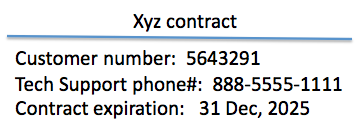
\includegraphics[width=70mm]{common/Figure-0.png}
\caption{Item}
\label{fig: Figure}
\end{figure}

\subsection{Shareable and Private Items}
There are two types of Items; Shareable and Private.
A Private Item cannot be shared with others while a Shareable Item can be shared.

%\subsubsection{Notes}
\section{Notes}
A Note is a special type of Item. It is similar to a sticky note (or postit note). 
A Note is a secure encrypted representation of its sticky note equivalent.
Every Note has a name. A Note also has a field that stores the content of the Note. 
Obidos provides a main menu option to manage Notes as 'standalone' Items since Notes are very commonly used, 
Standalone Notes are free standing Notes and can be created as Private or Shareable. Notes are the only free standing Items in Obidos.

\begin{figure}[H]
\centering
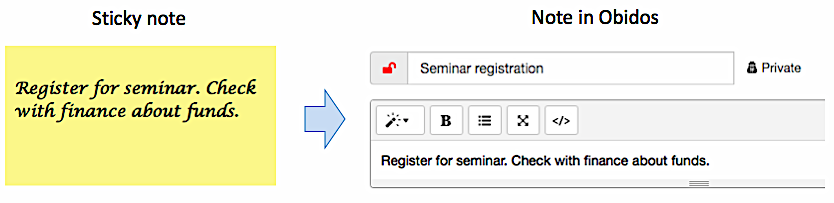
\includegraphics[width=120mm]{common/Note.png}
\caption{Note}
\label{fig: Figure}
\end{figure}

%\subsection{Containers}
\section{Containers}
Items stored inside Obidos can be organized into Containers. Each Container has a name.
For example, a Container named 'Personal Items' can be created to hold Items that are personal in nature.

There are two types of Containers; Private and Shareable.
Shareable Containers can be shared with others while Private Containers cannot be shared. 
By default, every user gets a Private Container called 'Private' and a Shareable Container called 'Public'. 

Each Container holds the Items stored in it.
Placing of an Item in a Container is dictated by the type of the Container and the type of the Item.

Private Containers can hold only Private Items. A Shareable Item cannot be placed in a Private Container.
Shareable Containers can hold both Shareable and Private Items (see Figure 1.3).

\begin{figure}[H]
\centering
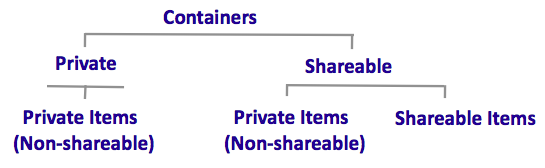
\includegraphics[width=90mm]{common/Figure-1.png}
\caption{Containers}
\label{fig: Figure}
\end{figure}

When a Shareable Container is shared with others, only Shareable Items inside the Container will be visible to them.
Private Items inside that Shareable Container will be completely hidden from others.

As an example, a Private Container named 'Personal Items' can be created to contain 3 Private Items 
named 'Bank Account', 'Cloud Account', and 'Procurement Card'. Note that in this case all the three Items will be Private
because a Private Container can hold only Private Items.

In addition to having a name, each Item is made up of field(s) and value(s).
For example, in the 'Personal Items' container, the 'Bank Account' Item can have a field 
'Account\#' with value '87399901".
In case the Routing number of the bank has to be stored, another field 'Routing\#'
can be added with its value '3452327'. (See figure 1.4)

\begin{figure}[H]
\centering
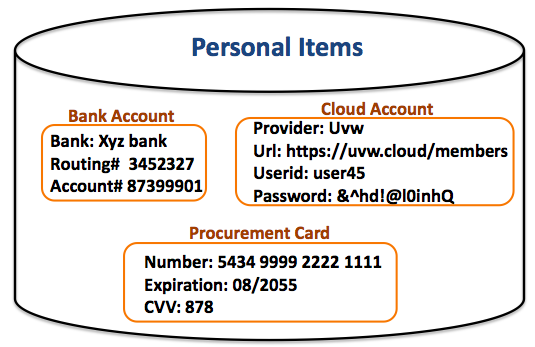
\includegraphics[width=80mm]{common/PersonalItems.png}
\caption{Private Container}
\label{fig: Figure}
\end{figure}

A Shareable Container named 'Lab Accounts' can be used to hold Shareable Items that has names 'xyz customer support' and 'Web Console'.
'Lab Accounts' Container may also hold a Private Item 'Database Account'.
When 'Lab Accounts' is shared to others, they will see the Items 'xyz customer support' and 'Web Console', but
will not see the Item 'Database Account'. (See figure 1.5)

\begin{figure}[H]
\centering
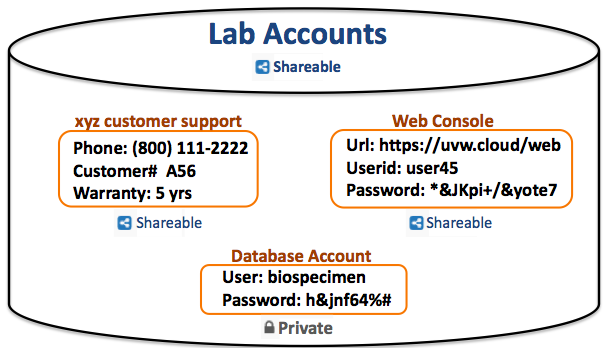
\includegraphics[width=80mm]{common/Lab-Accounts.png}
\caption{Shareable Container}
\label{fig: Figure}
\end{figure}

Users have permissions to create/modify Containers and Items. The distinction between standalone Notes and Containerized Items is visually represented in the following figure.

\begin{figure}[H]
\centering
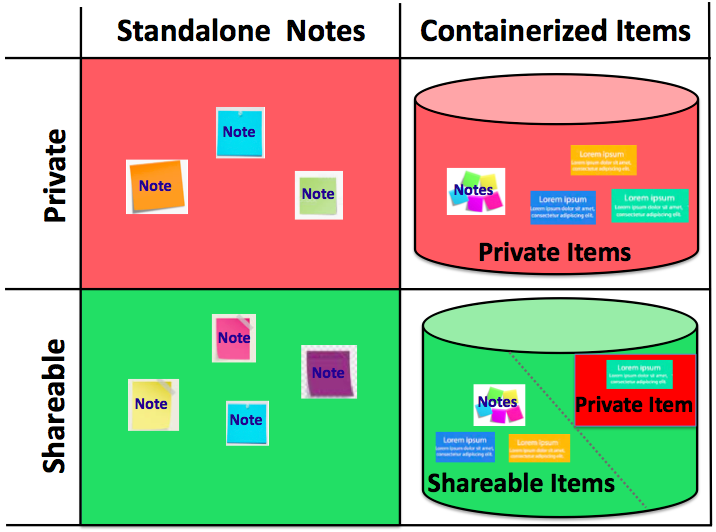
\includegraphics[width=80mm]{common/Standalone-Container.png}
\caption{Standalone Notes and Containerized Items}
\label{fig: Figure}
\end{figure}

\section{Templates}
There are various Items that follow a common format. Such formats can be captured as Templates.
Templates provide common structures for often used Items. A Template has the pre-defined fields of the Item.
These Templates can be used as a guide to create instances of Items in a Container.
When using a Template to create an Item, the User has to just fill in the values for the predefined fields.
Templates can be Global or Personal. Global Templates are available to all users.
Obidos provides a number of predefined Global Templates. 

For example, a Template called 'Cloud Account' can have the following fields:
  \newline \tab \tab url, username, password, email

When a user uses the 'Cloud Account' Template to create an Item called 'Web Server', values for the fields
url, username, password and email have to be supplied by the User (see following Figure).

\begin{figure}[H]
\centering
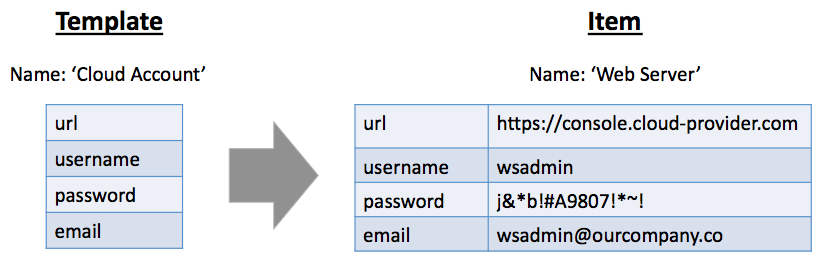
\includegraphics[scale=0.5]{common/Template-Item.png}
\caption{Instantiation of an Item from a Template}
\label{fig: Figure}
\end{figure}

Every user has permissions to create/modify Personal Templates.
However, creation/modification of Global Templates requires special permission.
The administrator can grant a user permission to create/modify Global Templates.
Users can also copy a Global Template into their Personal Templates and modify it to suit their purpose.

\section{Groups}
A set of users can be organized into a Group. The Group can have a name. It is possible to share an entity with a Group.
This makes it easy to share with a collection of users; especially if sharing is done to the same Group for multiple entities.

\section{Features}
Note that all features of Obidos are discussed in the guides. However, only the features that are licensed will be 
available in the instance.


    % -------------------------------------------------------------------------------------
    % INCLUDE All the chapters
    % -------------------------------------------------------------------------------------
   \chapter{Logging into Obidos}

The default login screen is shown in the following figure.

\begin{figure}[H]
\centering
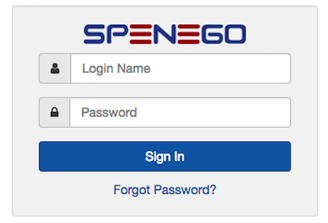
\includegraphics[scale=1.0]{user/Login-Screen.png}
\caption{Obidos Login Screen}
\label{fig: Figure}
\end{figure}

\section{Username and Password}
In order to log into Obidos a user needs a username and password.
If the user account is maintained completely within Obidos, it is a local account.
For local accounts, the username and password are both managed within Obidos.

If the user account is set up for single signon using corporate directory service,
the username and password must be entered as they are in the corporate directory.

\subsection{Local Password}
User passwords issued by Obidos will follow the password policies set in Obidos.
Initially the Administrator will set a temporary password.
The Administrator can choose to send an email to the User informing that an account has been created.
The first time the User logs in using temporary password, Obidos will prompt the User to set
permanent password that conforms to the password policy.

\begin{figure}[H]
\centering
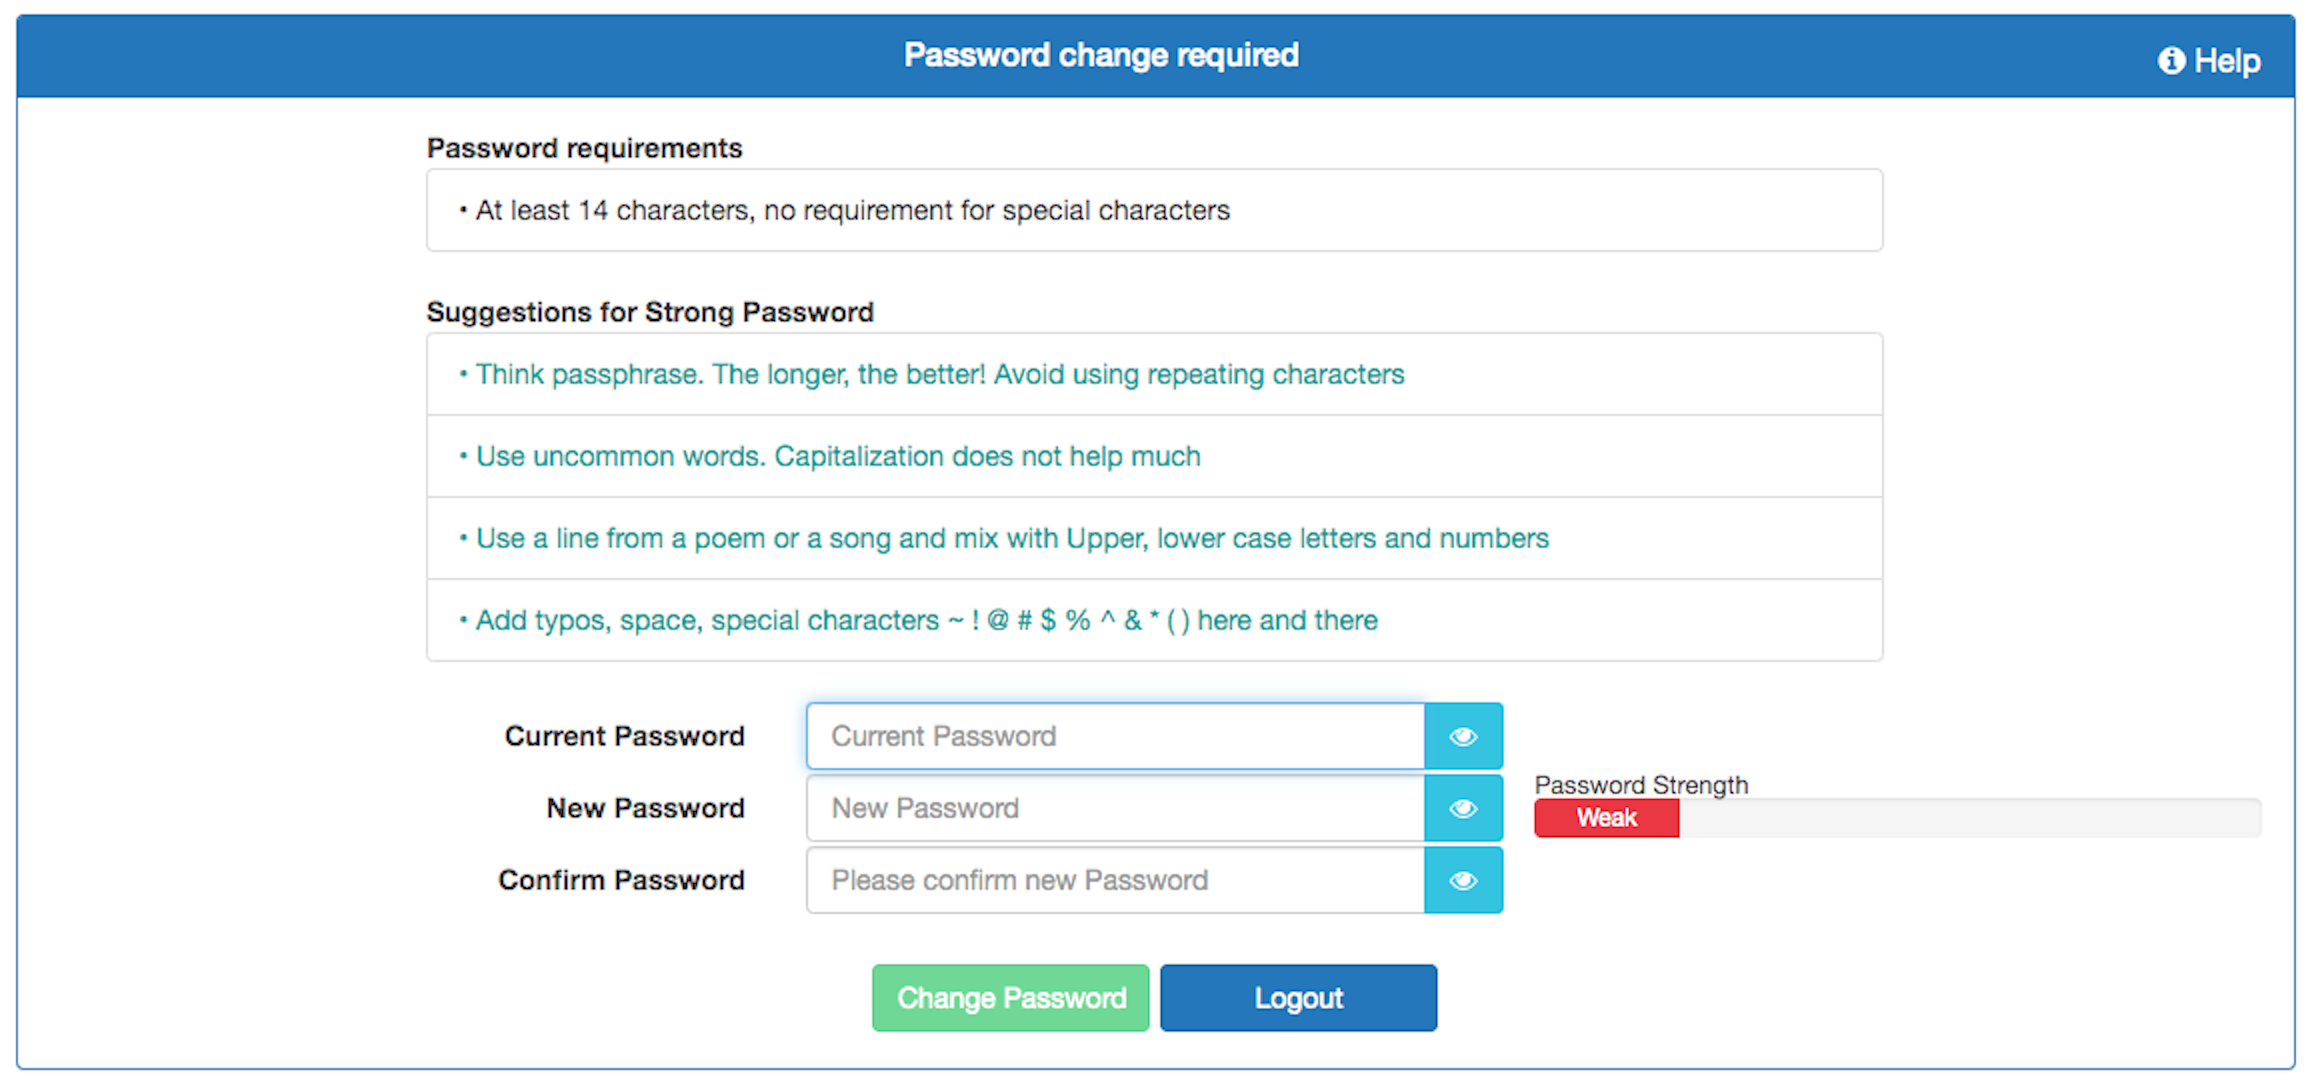
\includegraphics[scale=0.4]{user/Change-Temp-Password.png}
\caption{Change Temporary Password}
\label{fig: Figure}
\end{figure}

Once the new password is set, the User will be logged out of Obidos and prompted to log in using the new password.

\subsection{Directory-synchronized Password}
If a user password is synchronized with the corporate directory service, Obidos will
pass the User credentials to the corporate directory service to be validated.
In this case, Obidos do not have any control on the password.

\section{Passphrase}
When an Item is stored in Obidos, it is encrypted using one key from the personal key pair and
when the Item is retrieved, it is decrypted using the other key.
Such a private key pair is personalized using a passphrase that is chosen by the User.
Passphrase is a string that the User selects.
These passphrases are not stored in Obidos. The user will have to remember the passphrase.
Obidos will generate key pair (private \& public) for each user using the User's passphrase.
In order to retrieve an Item stored in Obidos, the User will need to provide the passphrase.
\textcolor{red}{If the User forgets the passphrase, it is not possible to retrieve any Item stored in the User's Containers.}

When logging into Obidos for the very first time, a user will be prompted to set the passphrase as shown in the following Figure. 

\begin{figure}[H]
\centering
%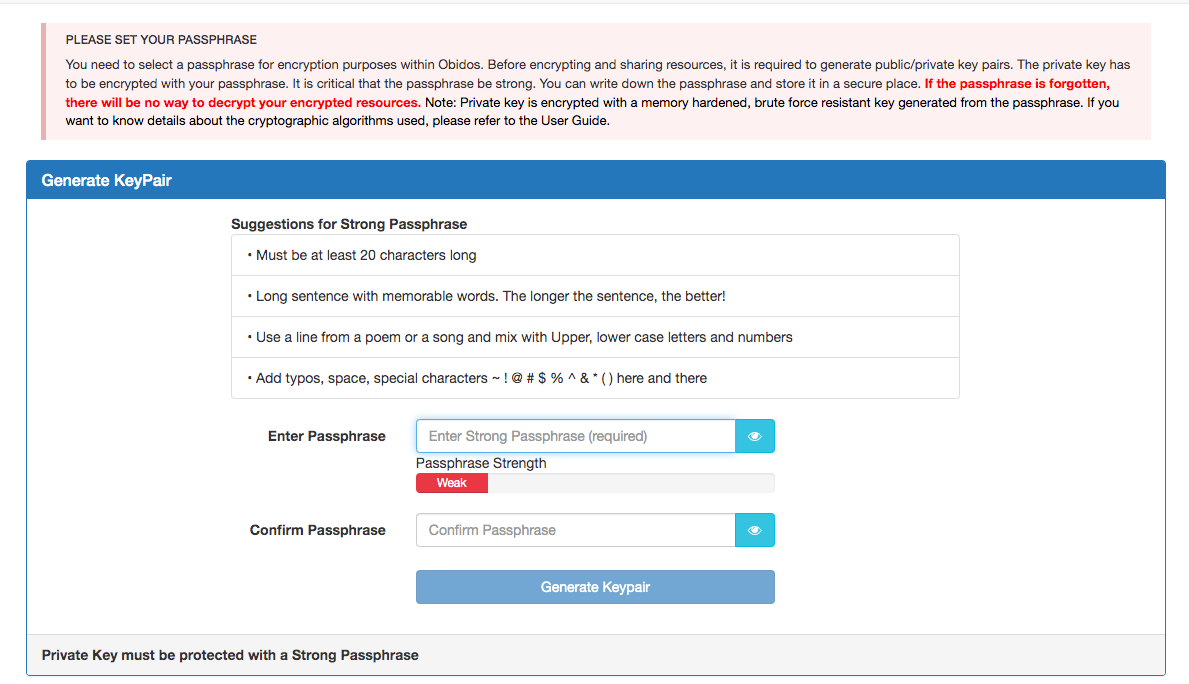
\includegraphics[width=90mm]{user/New-passphrase.png}
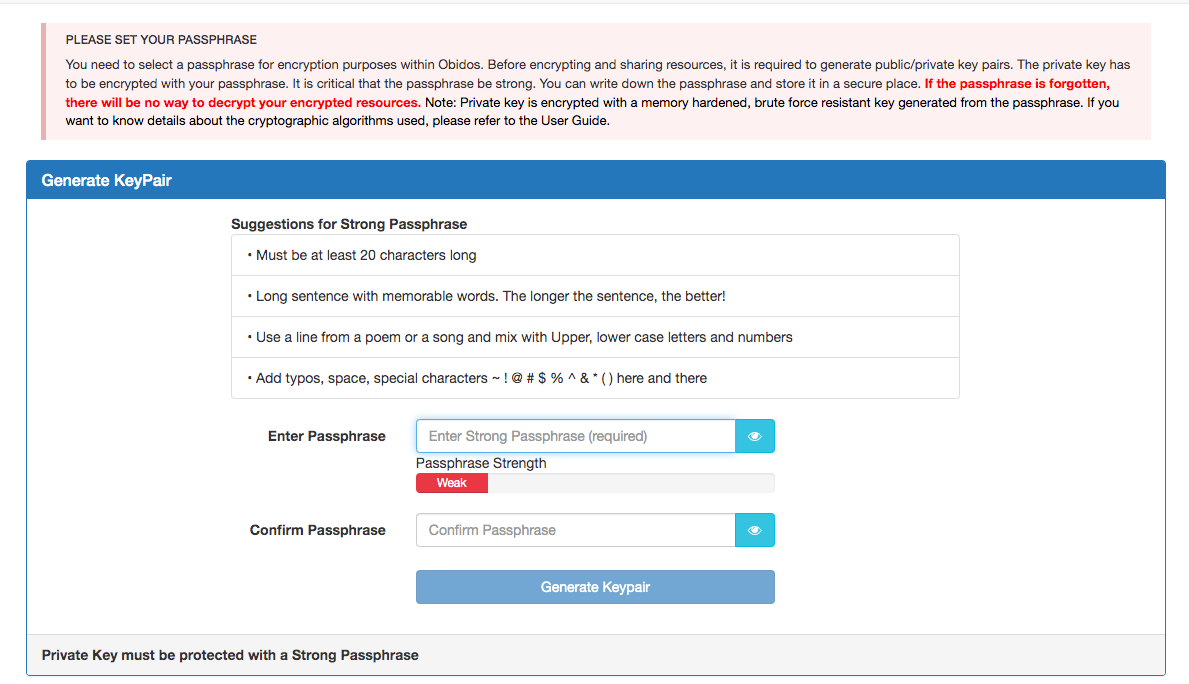
\includegraphics[scale=0.4]{user/New-passphrase.png}
\caption{Set New Passphrase}
\label{fig: Figure}
\end{figure}

A session is defined as the series of user interactions within Obidos once logged in till logout. 
The user can perform various activities during a session. 
Activities such as viewing an Item, sharing an Item, etc. requires the passphrase of the User. 
Instead of repeatedly entering the passphrase for each and every activity in the session, the User can provide the passphrase once for that session.
When a user logs into Obidos, there is an option to supply the passphrase for that session (see next Figure).
The session ends when the User logs out voluntarily or gets logged out by Obidos after a predefined period of inactivity.


\begin{figure}[H]
\centering
%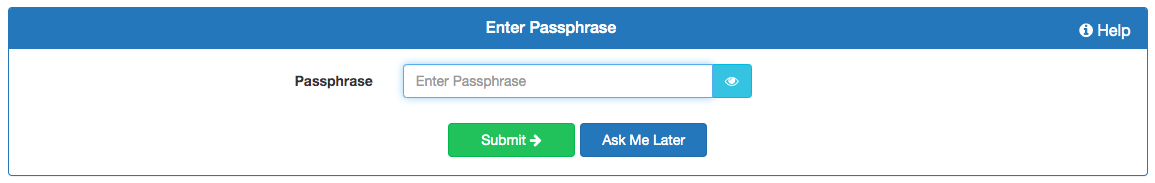
\includegraphics[width=90mm]{user/Login-Passphrase.png}
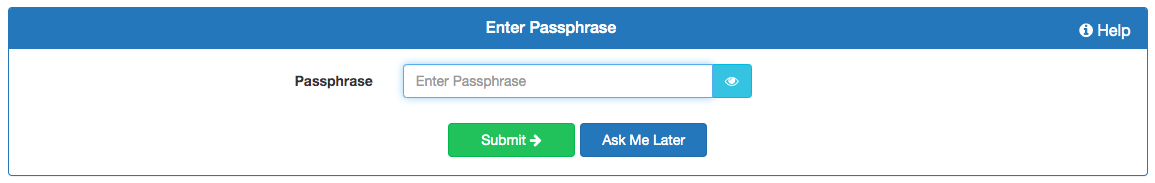
\includegraphics[scale=0.4]{user/Login-Passphrase.png}
\caption{Session Passphrase Activity}
\label{fig: Figure}
\end{figure}

If the passphrase is provided at the time of logging in, the User does not have to provide the passphrase
again for activities during that session.
If the passphrase is not provided at the time of logging in, the User can provide the passphrase at a later
point during the session.

Details of changing passphrase are given in the Chapter "Personal Preferences and Options".

\section{Logging Out}

The user can log out from a session using the Logout Menu Item from top right panel.

\begin{figure}[H]
\centering
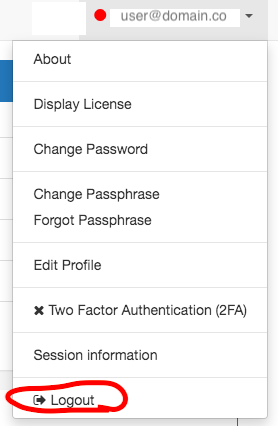
\includegraphics[scale=0.4]{user/Logout.png}
\caption{Logout menu}
\label{fig: Figure}
\end{figure}

In case there is no activity in the session for 30 minutes, the session will timeout and the User will be presented with a warning.

\begin{figure}[H]
\centering
%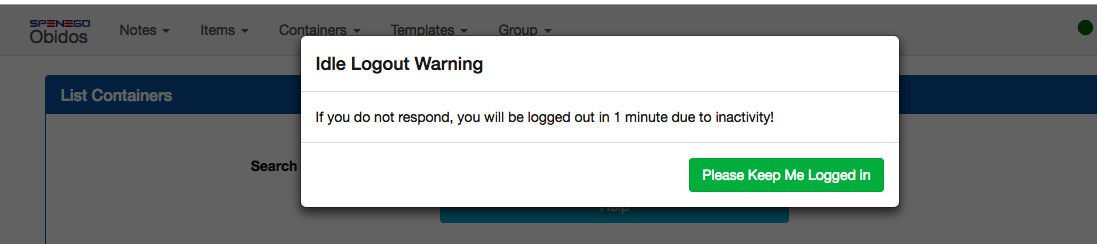
\includegraphics[width=90mm]{user/Inactivity.png}
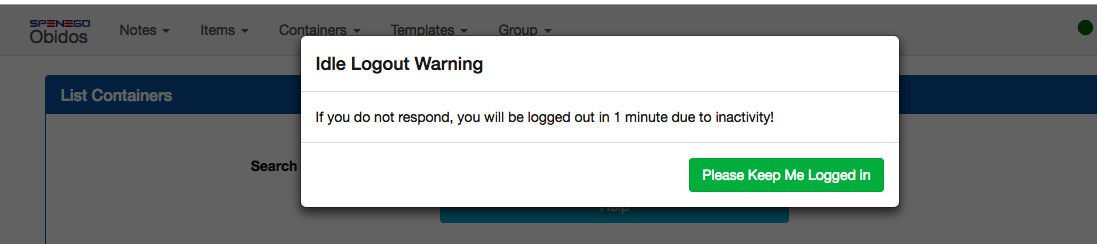
\includegraphics[scale=0.4]{user/Inactivity.png}
\caption{Inactivity Warning}
\label{fig: Figure}
\end{figure}

If the User fails to respond, the system will log out the User.


   \chapter{Password Strength}

The password strength is determined by calculating entropy of the 
password. An entropy is described in terms of bits. The higher the bits in entropy
the stronger the password will be. An entropy indicates how hard it will be to 
crack the password by brute-force. In password strength calculation, the entropy 
is not the same entropy as described in information theory. Rather the raw entropy 
is lowered by using various password cracking techniques before accepting.

\section{Understanding Password Entropy}
Entropy in password security measures the unpredictability and strength of a password. There are two main approaches to calculating password entropy:
\begin{enumerate}
    \item \textbf{Raw Entropy}: This method calculates entropy based solely on the password's length and character set. It often results in higher entropy values, which some password strength tools use.
    
    \item \textbf{Adjusted Entropy}: Our tool uses this more nuanced approach. We start with the raw entropy, then apply various reduction techniques to account for real-world password vulnerabilities.
\end{enumerate}

\section{Why Our Entropy Scores Might Seem Lower}

Our tool provides a more conservative and realistic assessment of password strength. We apply several techniques to reduce the initial entropy, including:

\begin{itemize}
    \item NIST Special Publication 800-63 guidelines
    \item Weakening for repeated characters
    \item Adjustments for lowercase-only passwords
    \item Qwerty keyboard pattern recognition
    \item Dictionary word detection
    \item Leet speak translation (e.g., ``@'' to ``a'')
    \item Keyboard pattern adjustments
\end{itemize}
For example, in our tests:
\begin{itemize}
    \item ``Tr0ub4dor\&3'' has a raw entropy of 72.27, but an adjusted entropy of 19.63
    \item ``correcthorsebatterystaple'' starts at 117.51 and adjusts to 30.95
    \item ``password'' goes from 37.60 to 2.0
\end{itemize}

These adjustments reflect real-world vulnerabilities that attackers might exploit, providing a more accurate representation of your password's strength against modern cracking techniques.

While our entropy scores may appear lower than other tools, they offer a more realistic assessment of your password's security in practical scenarios. Always aim for higher entropy scores and follow good password creation practices for optimal security.

\section{Entropy Calculation}
This section describes the basics of entropy calculation. Please note that we
do not calculate password or passphrase entropy this way, rather we
use various password cracking techniques to lower the raw entropy and if the
entropy is higher or equal to the configured entropy, only then the password
is accepted.

If the password length is $L$ and the password can be chosen from $N$ number of
characters, the possible number of passwords will be $N^L$. To calculate the raw 
entropy $H$ in that character space, the $H$ has to be a number so that
$2^H = N^L$. Therefore, the entropy calculation formula can be derived as follows:

\begin{align}
                 2^H &= N^L\label{eq:1} \\
           \log(2^H) &= \log(N^L)\label{eq2}\\
    H \times \log(2) &= L \times \log(N)\label{eq:3}\\
                   H &= L \times \frac{\log(N)} {\log(2)}\label{eq:4} \\
                     &= L \times \log_{2}(N)\label{eq:5}
\end{align}
\footnotetext[1]{$\log{_b}(x^p) = p\log{_b}(x)$}
\footnotetext[2]{$\log_{b}(x) = \frac{\log(x)}{\log(b)}$}

Given a password entropy $H$ and the number to guess a password per second is ($gps$), the time in seconds
$T_{s}$ to brute force a password can be calculated with the following formula:

\begin{align*}
    T_{s} &= \frac{2^H} {gps}
\end{align*}

The following xkcd comic illustrates entropy calculation of password in a 
different way.

\begin{figure}[H]
    \centering
    \fbox{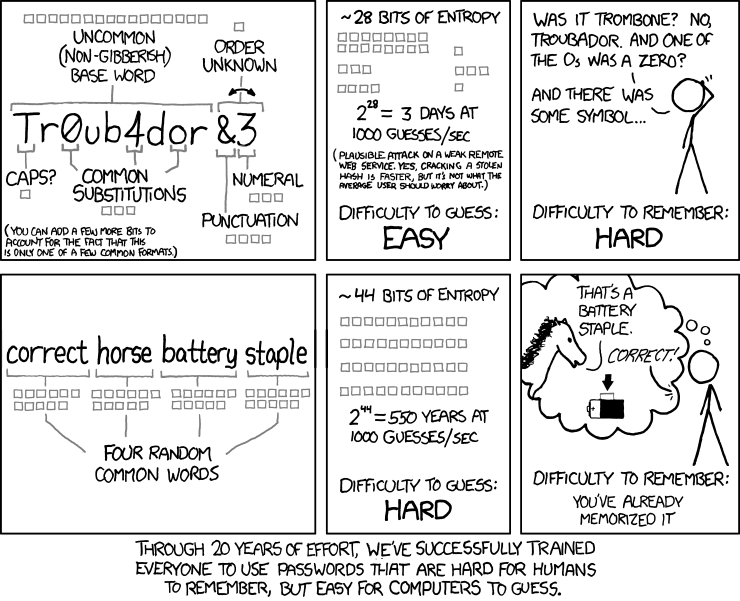
\includegraphics[scale=0.6]{common/xkcd_password_strength.png}}
    \caption{xkcd comic for password strength}
    \label{fig: Figure}
\end{figure}

Let's calculate the entropy of \texttt{Tr0ub4dor\&3} with our formula
$H = L \times \log_{2}(N)$. The password has upper case, lower case, numbers and a 
special character in it. There are 26 upper case, 26 lower case, 10 numbers and
32 special characters (including space) in English keyboard and the length $L$ of the password is 
$11$. 

\begin{align*}
    N &= 26 + 26 + 10 + 32 = 94 \\
    H &= 11 \times \frac{\log(94)} {\log(2)} =  72.10047736845401109442 \approx 72
\end{align*}
Assuming that the attacker knows the length of the password $L$ and character
space $N$,
if $gps = 1000$, it will take $\frac{2^{72}} {1000}$ $\approx$ $150\ billion$ years 
to crack the password. If $gps =350\ billion$, it will take $\approx$ $428$ years to crack 
the password. if $gps = 1\ trillion$, it will take $\approx 150\ years$ to crack the
password. So if brute force is used, it is really a good password, even with the
most powerful computer, it will take a long time to crack. 

According to xkcd,
the password is not strong, lets see how xkcd calculates the entropy. Each of
the tiny square box in the comic indicates a bit. 
\begin{itemize}
    \item The $16$ bits implies that the word 
\texttt{Troubador} is chosen from a dictionary with $65536$ words ($2^{16} = 65536$).
    \item Make the first letter upper case, there is only $1\ bit$.
    \item Two characters were substituted $o \rightarrow 0$, $a \rightarrow 4$ and $o$ was
not substituted, therefore $3 bits$ of information.
    \item The string \texttt{\&3} was appended at the end. The order is unknown, therefore $1\ bit$
    \item There are 32 special characters (including space) in English keyboard, therefore the entropy should
be $1 \times \frac{\log(32)} {\log(2)} = 5$. For some reason $4 bit$ was selected.
\end{itemize}


Therefore, the entropy of \texttt{Tr0ub4dor\&3} is $ 16 + 1 + 3 + 1 + 4 + 3 = 28$, which much 
is lower than 72 and makes it a bad password, because the attacker might follow
the similar technique than brute-forcing it.

\section{Entropy calculation in Obidos}
The technique we used in Obidos, the entropy for the password \texttt{Tr0ub4dor\&3}
comes down to 19.625. we used similar techniques used the ruby gem 
\href{https://github.com/bdmac/strong_password}{strong\_password}

\begin{enumerate}
    \item Calculate entropy according to
\href{https://nvlpubs.nist.gov/nistpubs/Legacy/SP/nistspecialpublication800-63ver1.0.2.pdf}{NIST Special Publication 800-63 Version 1.0.2} Appending A.2.1
    \begin{itemize}
        \item The first character gets 4 bits
        \item The next 7 characters get 2 bits/character
        \item The next 12 characters (9-20) get 1.5 bits/character
        \item Any character beyond 20 gets 1 bit/character
        \item If there are mixed case and special character, give 6 bits bonus
    \end{itemize}
    Using these rules, the entropy of \texttt{Tr0ub4dor\&3} comes down to 26.125
    \item Calculate the entropy by lowering the case, which is also 26.125
    \item Adjust entropy by checking if the password has any pattern of 
Qwerty keyboard (e.g. zxcvbn, qwertyuiop etc.) which is 26.125
    \item Adjust the entropy by looking at dictionary, doing normal
substitutions like xkcd, checking for leet speak pattern etc. The entropy comes down
to 19.625.
    \item Finally select the lowest entropy, which is 19.625 
\end{enumerate}
The entropy of \texttt{correcthorsebatterystaple} comes down to 30.953125 which
is much lower than xkcd's 44 bit entropy.
\section{Suggestions for strong passwords}
Please think passphrase when picking a password. Passphrases are longer and 
easier to remember than a cryptic random password which is difficult to remember.
The longer the password is, the stronger it will be. Refer to the equation \eqref{eq:5}.
\begin{itemize}
    \item Think passphrase. The longer, the better! Avoid using repeating characters
    \item Use a line from a poem or a song and mix with Upper, lower case letters and numbers
    \item Use uncommon words. Capitalization does not help much
    \item Add typos, space, special characters \! \@ \# \$ \% \textasciitilde \ \textasciicircum \ \& \* \( \) etc. here and there.
If the password is a long passphrase, there is no requirement to use any 
special character. However, your organization might have a password policy 
that requires them.
    \item Do not use username, email, phone numbers etc.
\end{itemize}
\section{Password storage}
A password is never stored in the disk, rather a memory-hardened, brute-
force resisting key is derived from the given password and a stored salt. To verify a 
password, the same key is derived from the password and the salt and 
compared.  The function deriving the key from the password and
the salt is CPU intensive and intentionally requires a fair amount of 
memory. Therefore, it mitigates brute-force attacks by requiring a 
significant effort to verify each password. 

The password is hashed using
\href{https://github.com/P-H-C/phc-winner-argon2/raw/master/argon2-specs.pdf}{Argon2id} algorithm. 

   \chapter{Personal Preferences and Options}

There are some customizations that can be done on an individual basis. These options are available through the 
drop down menu on the top right side of the panel (see the highlighted red frame in the following figure).

\begin{figure}[H]
\centering
\fbox{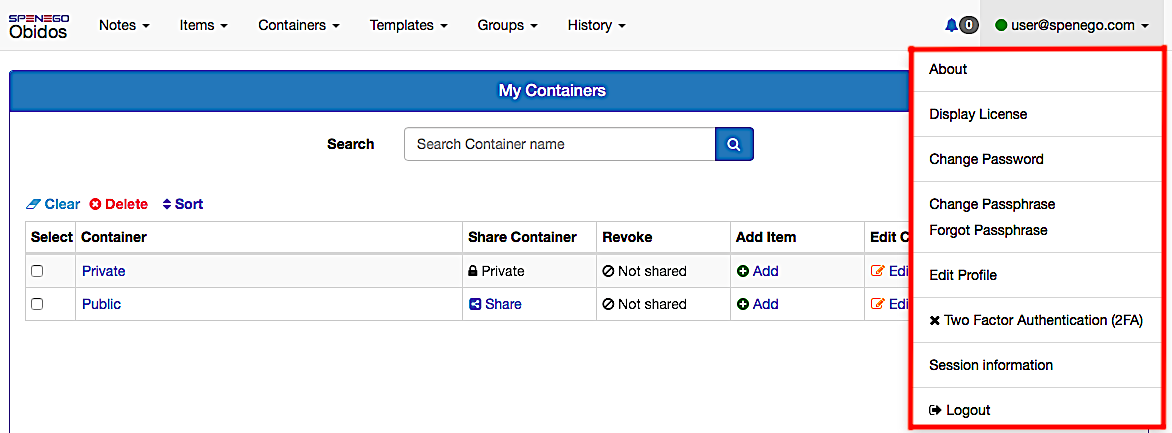
\includegraphics[scale=0.4]{user/Preferences.png}}
\caption{Preferences and Options menu}
\label{fig: Figure}
\end{figure}

\section{Display License}
The 'Display License' option shows your site license information for Obidos. 
The Open Source License has no expiration and supports any number of users. 
Standard and Enterprise Editions are annual subscription based. 
Once the license expires, users have 30 days of grace period
for using the software without interruption. During the 30-60 day period after license expiration, existing
entities can be viewed, but no new entities can be created. After 60 days of expiration, users will be
able to view only the license and their activity history; no other activities will be permissible.
List of all features available in each license edition is displayed in this screen.
\subsection{License Expiration}
30 days before the expiration of Obidos license, users will see warning message about license expiration.
This warning message will be displayed when the User logs into Obidos.
Once the license expires, users will have 30 days of grace period to use the software without disruption.
Between 30 days and 60 days after license expiration, users will not be able to create any new entities.
During this period, users can view their entities.
After 60 days of license expiration, they will not be able to use the software. A new license will need to be installed.
During the periods of disruption due to expired license, all user entities will remain intact in Obidos. 
Only with a valid license will users be able to use the software as usual.

\section{Change Password}
If the user account is local, then password can be changed using this option.

%\subsection{Changing Passphrase}
\section{Changing Passphrase}

If the User wants to change passphrase, it can be done through this option.
When the passphrase is reset, none of the existing entities owned by the User will be affected.

%\subsection{Forgotten Passphrase}
\section{Forgotten Passphrase}

\textcolor{red}{If the User forgets the passphrase, none of the stored Items can be retrieved.}
In this case, the User has two options. One is to reset the passphrase. The other is to create a new account
and start using Obidos from scratch.
If the User chooses to reset the passphrase, all the stored artifacts (Notes/Items/Containers) will be deleted and cannot be recovered. 
This is because Obidos will have to recreate a new key pair and overwrite the existing key pair.
Consequently, the previously stored artifacts (Notes/Items/Containers) cannot be recovered. Hence,
Obidos will delete those artifacts when the passphrase is reset.
An email with instructions for resetting the passphrase will be sent to the User. If the Administrator 
configured the account to use 2FA for passphrase reset, the User will be required to use 2FA as part of resetting
the passphrases.

If the User chooses to get a new account and start from scratch, all Notes/Items/Containers in the old account
will remain intact. If the User manages to remember/recover the passphrase for the old account even after creating a new account, 
it can be used as usual.
Note that it is not possible to merge the Notes/Items/Containers in two accounts.
Although, the User has the option to share Shareable Notes/Items/Containers from one account to the other and 
thus retrieve the contents of Shareable Notes/Items/Containers from one account; but this won't help in the case of Private Containers.


%\subsection{Edit Profile}
\section{Edit Profile}

The user can load a profile picture using the 'Upload new profile picture' button.
The profile picture can be deleted by using the 'Delete profile picture' button.

\begin{figure}[H]
\centering
\fbox{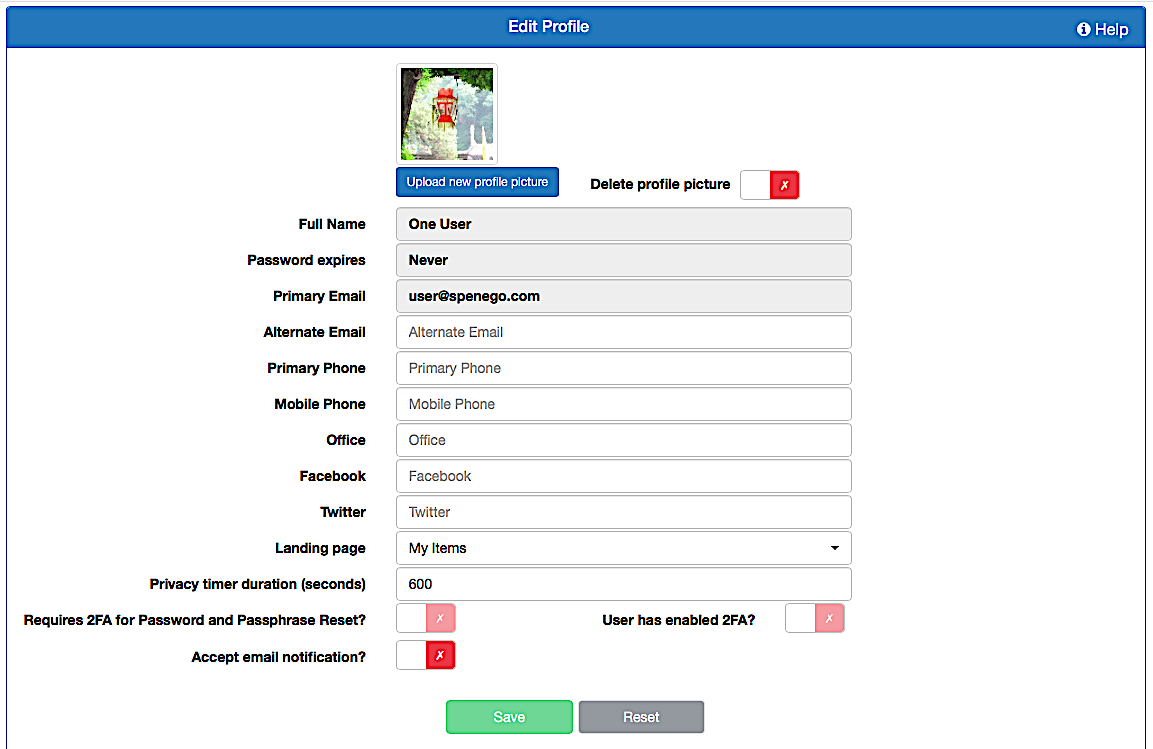
\includegraphics[scale=0.4]{user/User-profile.png}}
\caption{User Profile}
\label{fig: Figure}
\end{figure}

Alternate Email, Primary Phone, Mobile Phone, etc. are optional information.
\newline
\newline
'Landing Page' is the first page the User sees when logged in. The Landing page can be set to 'My Notes', 'My Items',
'My Containers', etc.
\newline
\newline
'Privacy timer duration' is the amount of time in seconds that an Item will be displayed for viewing.
The privacy timer starts as soon as an Item is displayed. At the end of the specified seconds, the Item will be hidden.
If you set the 'Privacy timer duration' to 0, then the timer will be off. 
\newline
\newline
The 2FA entries are only for information.
\newline
\newline
'Accept email notification?' flag is used by Obidos to screen email notifications. When a user shares an Item/Note/Container
with another user, the sender has the option to send an email notification to the recipient. 
Such notifications can be stopped by setting 'Accept email notification?' to x.

\section{Notifications}
Obidos has an internal notification system. This mechanism will notify the User when someone is sharing an entity 
or some user capabilities have been updated. Such notifications can be seen once the User logs into Obidos.

\begin{figure}[H]
\centering
\fbox{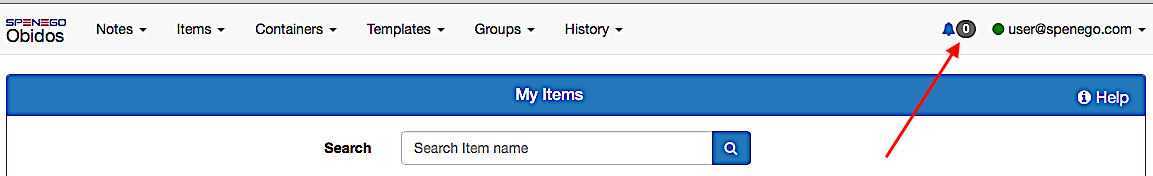
\includegraphics[scale=0.4]{user/Notifications-start.png}}
\caption{Notifications Status}
\label{fig: Figure}
\end{figure}

When notifications are present, the count will be displayed inside the red circle at the top right.
Clicking on the red circle will open up the 'Notification Messages' window.

\begin{figure}[H]
\centering
\fbox{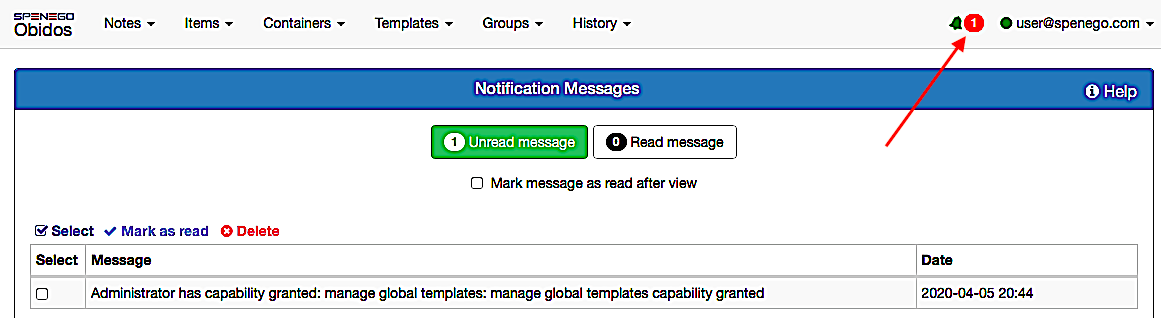
\includegraphics[scale=0.4]{user/Notifications-present.png}}
\caption{Notification Messages}
\label{fig: Figure}
\end{figure}

Some notifications are read only informational messages, while others are information links
that can be clicked on so that the entity referred in the message can be viewed.
If a notification is to be deleted, select the notification using the checkbox on the left and click on the
{\color{red}\faTimesCircle \ Delete} button.

   \chapter{General Features}

\section{Sharing}
A Shareable Container or Item or Note can be shared with other user(s). An entity that needs to be shared has to be tagged as Shareable when it is created. This is because a Private entity cannot be shared.

\section{Revoking Sharing}
The sharing of a Container/Item/Note can be stopped by revoking. When the sharing is revoked, the recipient(s) will no longer have access to the shared entity.

\section{Expiring Sharing}
It is possible to set an expiration date on the sharing of a Container/Item/Note. After the expiration date, the expired entity will not be visible to anyone other than the owner. The expiration date can be changed at will by the owner of the entity.

\section{Granting Permissions}
The owner of a Container/Item/Note can share it with another user. When it is shared, the recipient will get
only permission to 'view' the artifact. The owner can grant two special permissions to the recipient. One is 'update' and the other is 'own'. When the recipient is granted update permission, the recipient can edit the artifact. If the recipient is granted 'own' permission, then the recipient can take ownership of the artifact. Once the ownership is taken over by the recipient, the original owner will only have view permissions.

There are some features and menus that are commonly available in various screens in Obidos. 
These are outlined here for easy reference.

\section{Help Menus}
\subsection{Top Level Menus}
There are 6 top level menus in Obidos. They are Notes, Items, Containers, Templates, Groups and History. 
Each of these top level menus has a Help selection. This Help page covers aspects of operations 
within that top level menu at a high level.

As an example, looking at the Notes top level menu, there is a Help menu for Notes (see following Figure).

\begin{figure}[H]
\centering
\fbox{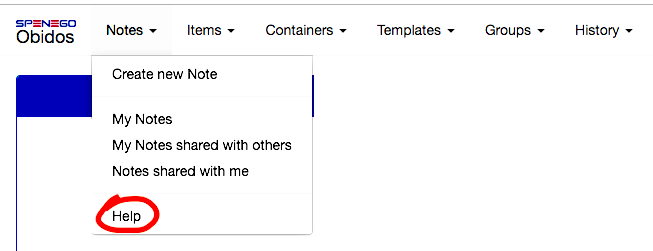
\includegraphics[scale=0.35]{user/Note-Help.png}}
\caption{Main Help for 'Notes' top level menu}
\label{fig: Figure}
\end{figure}

Similarly, for the Containers top level menu, there is a Help menu for Containers.

\begin{figure}[H]
\centering
\fbox{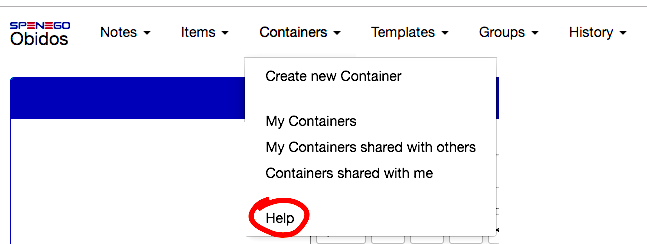
\includegraphics[scale=0.35]{user/Container-Help.png}}
\caption{Main Help for 'Containers' top level menu}
\label{fig: Figure}
\end{figure}

\subsection{Screen Level Menus}
Every screen has a Help section.
This Help section is accessible by clicking on the 'Help' button at the right of the blue header bar.
(See the red circled area in the following Figure).

\begin{figure}[H]
\centering
\fbox{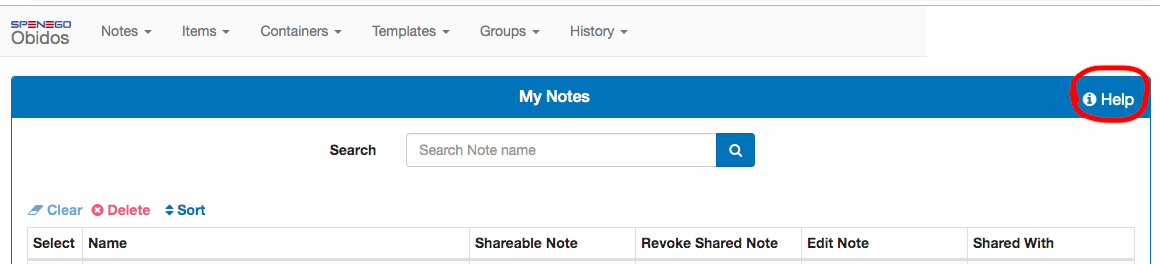
\includegraphics[scale=0.35]{user/List-Notes-Help.png}}
\caption{Screen level Help}
\label{fig: Figure}
\end{figure}

This screen level Help is a toggle button. When you click on the Help button, the help section will
open up at the top of the page. Clicking on the Help button again will collapse the help section. 

\section{Action Icons}

In many of the sections to follow, you will come across the following icons. Each one of these icons represent
a specific action that can be performed on the artifact in context. 
Some icons are reused in different scenarios with different colors.
These icons are listed here for easy reference.
\newline

\begin{center}
    \begin{tabular}{ | c | c | c | }
        \hline
        \textbf{Icon} & \textbf{Meaning} & \textbf{Description} \\
        \hline
            {\color{mygreen}\faPlusCircle} & Add & Add an Item to Container \\
        \hline
            {\color{myblue}\faEraser} & Clear & Clear the selections made \\
        \hline
            {\color{red}\faTimesCircle} & Delete & Delete the selected entities \\
        \hline
            {\color{orange}\faEdit} & Edit & Edit the entity in context \\
        \hline
            {\color{red}\faClockO} & Expired & This Note or Item has expired \\
        \hline
            {\color{red}\faEyeSlash} & Hide & Hide the Note or Item currently viewed \\
        \hline
            {\color{myblue}\faUsers} & List & List users and groups the entity is shared with \\
        \hline
            {\color{mygray}\faBan} & None or Not Allowed & The current activity in context is Not allowed \\
        \hline
            {\color{red}\faUnlock} & Not Secure & Value of this field is stored in plain text \\
        \hline
            {\color{mygray}\faLock} & Private & This entity is tagged as Private \\
        \hline
            {\color{orange}\faBan} & Revoke & Revoke sharing the entity in context \\
        \hline
            {\color{mygreen}\faLock} & Secure & Value for this field is stored encrypted \\
        \hline
            {\color{myblue}\faShareAltSquare} & Share & Share this artifact with others \\
        \hline
            {\color{mygray}\faShareAlt} & Shareable & This entity is tagged as Shareable \\
        \hline
            {\color{myblue}\faShareSquare} & Shared & Shows that the entity is shared with some user(s) \\
        \hline
            {\color{myblue}\faSort} & Sort & Sort the list of entities \\
        \hline
            {\color{mygreen}\faEye} & View & View the currently hidden Note or Item \\
        \hline
            {\color{mygreen}\faClockO} & Will Expire & This Note or Item has an expiration set on it \\
        \hline
    \end{tabular}
\end{center}

\section{Lengths of Entries}

The following table summarizes the maximum number of input characters allowed when creating various entities.
\begin{center}
    \begin{tabular}{ | c | c | }
        \hline
        \textbf{Identifier} & \textbf{Max number of characters} \\
        \hline
            Name (Note,Item,Container etc.) & 64 \\
        \hline
            Template field & 32 \\
        \hline
            Comment field & 256 \\
        \hline
    \end{tabular}
\end{center}

\section{Navigation in Listings}

Navigation through the listing menus are similar and described here.
\newline
By default, the entities (Notes/Items/Containers/Templates/Groups) will be displayed in the order in which they were created with the latest one at the top.
To sort the list of entities in another order, click on {\color{myblue}\faSort} \textcolor{myblue}{Sort} icon above the list bar.
The sort menu will show up and you can sort based on those options.

\begin{figure}[H]
\centering
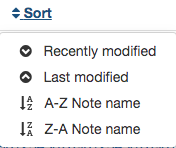
\includegraphics[scale=0.5]{user/Sort-Menu.png}
\caption{Sort Menu Options for Items}
\label{fig: Figure}
\end{figure}

The number of entities that exist can be seen at the bottom of the screen.
For example if there are 23 entities and 14 are listed in the current screen, at the bottom of the screen you will see 

\begin{center}
{\color{myblue}\faStepBackward} {\color{myblue}\faChevronCircleLeft} 1-14 of 23 
{\color{myblue}\faPlayCircle} {\color{myblue}\faStepForward}
\end{center}

In order to move forward in the list one at a time, click on {\color{myblue}\faPlayCircle}.
To move forward a complete page, click on {\color{myblue}\faStepForward}.
Similary, to go back in the list one at a time, click on {\color{myblue}\faChevronCircleLeft}.
and to go back one complete page, click on {\color{myblue}\faStepBackward}.

   \chapter{Notes}

A Note is similar to a postit note. A Note has only two parts - name and content.
The name of a Note is the identifier used for display purposes. The name can also be used to search for a Note of interest.
The content is the textual information in the Note.
A Note can be standalone or placed inside a Container. In this section we are explaining the operations associated with a standalone Note. However, the principles outlined here applies to a Note created as an Item inside a Container too.
Notes can be Private or Shareable.
A Private Note cannot be shared with any user.

\section{Create a Note}
From the top \textbf{Notes} menu, select \textbf{Create New Note}. The resulting screen will be as in the following figure:

\begin{figure}[H]
\centering
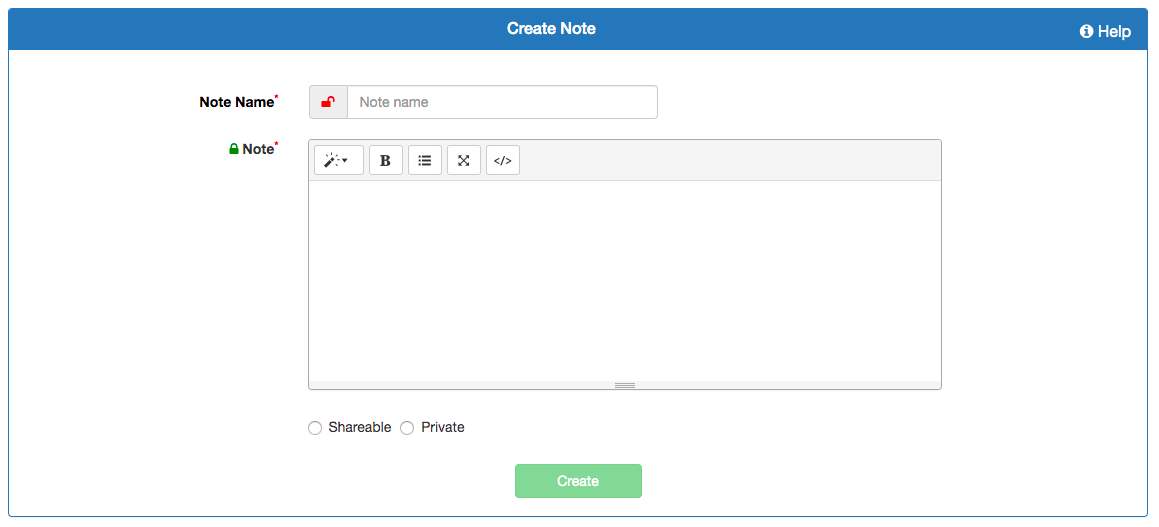
\includegraphics[scale=0.4]{user/Create-Note.png}
\caption{Create New Note}
\label{fig: Figure}
\end{figure}

When creating a Shareable Note, it is possible to set an expiration. The user can specify the date on which the Note will expire. 
Once a Note expires, it will not be accessible to the shared users/groups.
It is not possible to set expiration on a Private Note.

\section{List Notes}
Select \textbf{List My Notes} from the top level \textbf{Notes} menu.
The result with be similar to the figure shown below:

\begin{figure}[H]
\centering
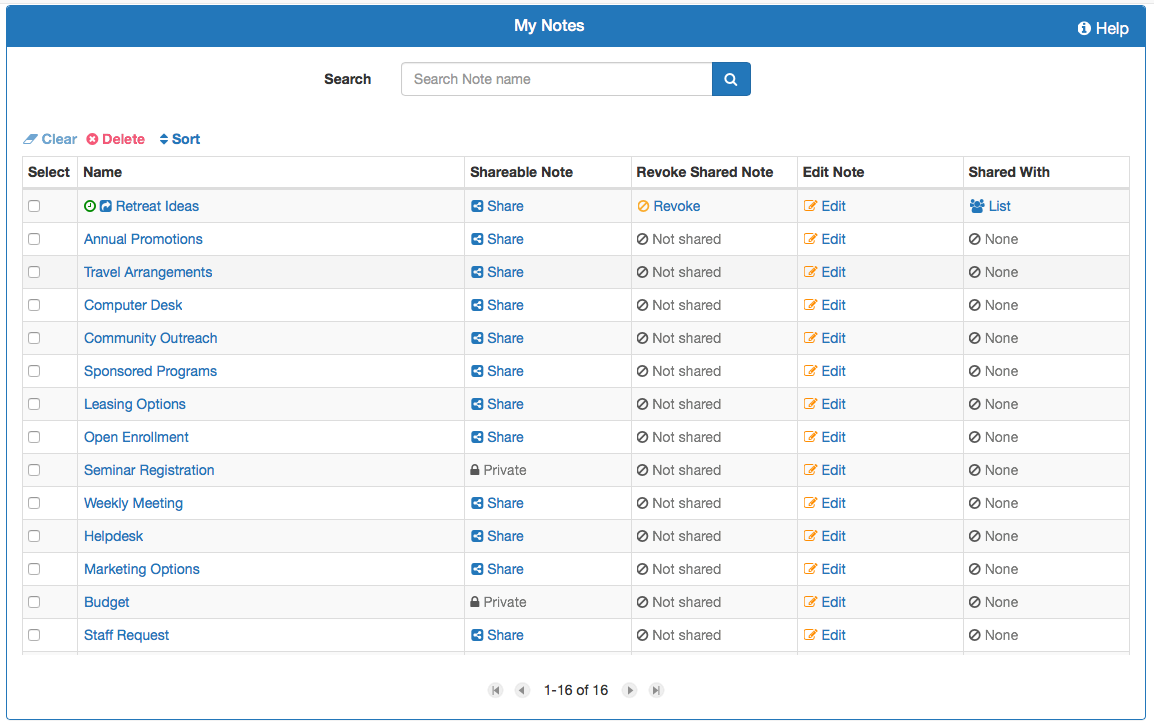
\includegraphics[scale=0.425]{user/List-My-Notes.png}
\caption{List My Notes}
\label{fig: Figure}
\end{figure}

The order of listing of Notes can be changed using the {\color{myblue}\faSort \ Sort} option.

\begin{figure}[H]
\centering
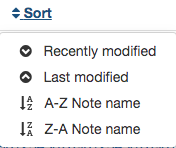
\includegraphics[scale=0.5]{user/Sort-Menu.png}
\caption{Sort Notes}
\label{fig: Figure}
\end{figure}

\section{View a Note}
Get the List of Notes (see section above). Click on the name of the Note to view it.

\begin{figure}[H]
\centering
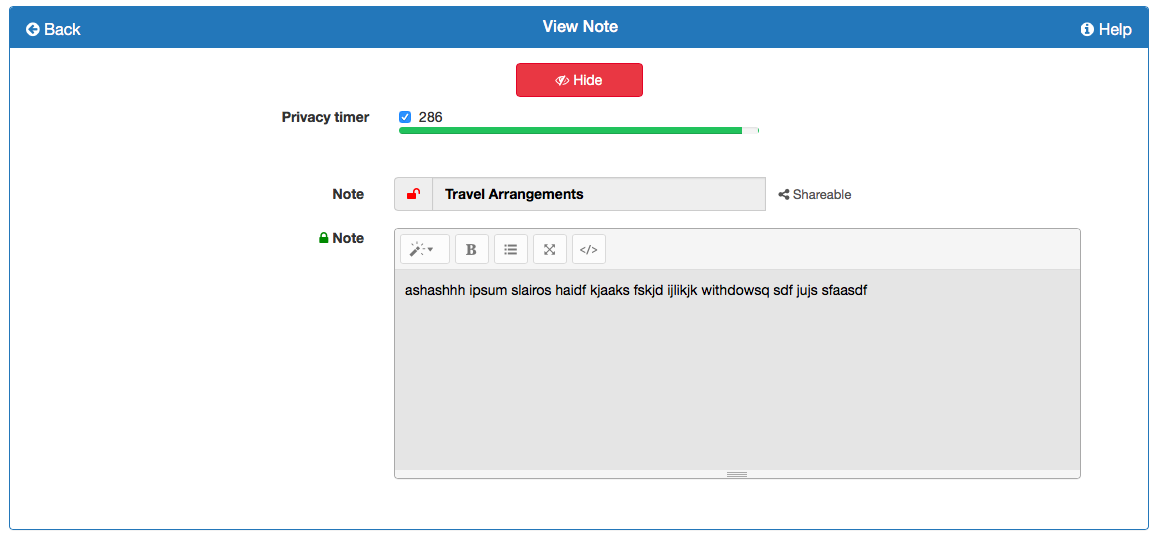
\includegraphics[scale=0.425]{user/View-Note.png}
\caption{View Note}
\label{fig: Figure}
\end{figure}

\section{Edit a Note}
From the List of Notes, a Note can be edited by clicking the {\color{orange}\faEdit} {\color{myblue}Edit} link.

\section{Delete a Note}
From the List of Notes, select the Note(s) to delete by clicking on the select button to the left of Note(s). 
Then click on {\color{red}\faTimesCircle \ Delete}. You will be asked to confirm the deletion. 

Note: When a Note is deleted, it will also be removed from all users to whom it was previously shared.

\section{Share a Note}
Sharing a Note can be done only from the List of Notes (see section above).
From the List of Notes, on the line corresponding to the Note, click on {\color{myblue}\faShareAltSquare \ Share} to initiate sharing of the Note.

   \chapter{Containers}

Containers hold Items created by the User.
A Container created as Private cannot be changed to Shareable.
Similarly a Shareable Container cannot be changed to a Private Container.

\section{Create a Container}

From the Menu bar on top, select "Containers" tab and then select "Create new Container" from drop down menu.

\begin{figure}[H]
\centering
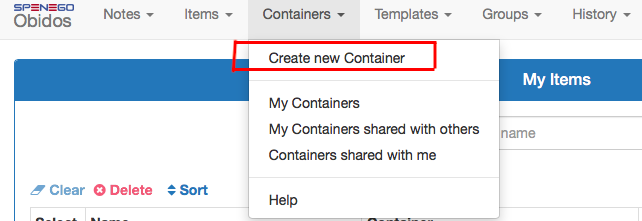
\includegraphics[width=90mm]{user/Create-Container.png}
\caption{"Create new Container" Menu}
\label{fig: Figure}
\end{figure}

In the 'Create Container' page, give a name for the Container. Specify the type of the Container, whether Shareable or Private. 

\begin{figure}[H]
\centering
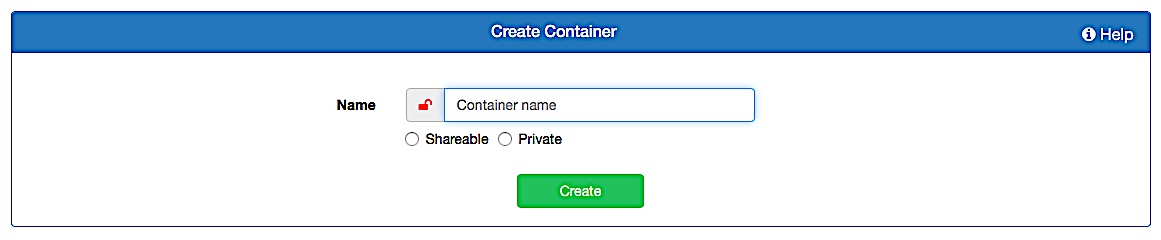
\includegraphics[width=150mm]{user/Create-Container-Frame.png}
\caption{Creating a Container}
\label{fig: Figure}
\end{figure}

\section{List Containers}

Select "My Containers" from the top "Containers" tab.
The list of Containers will be displayed in the format as shown in the following figure.

\begin{figure}[H]
\centering
\fbox{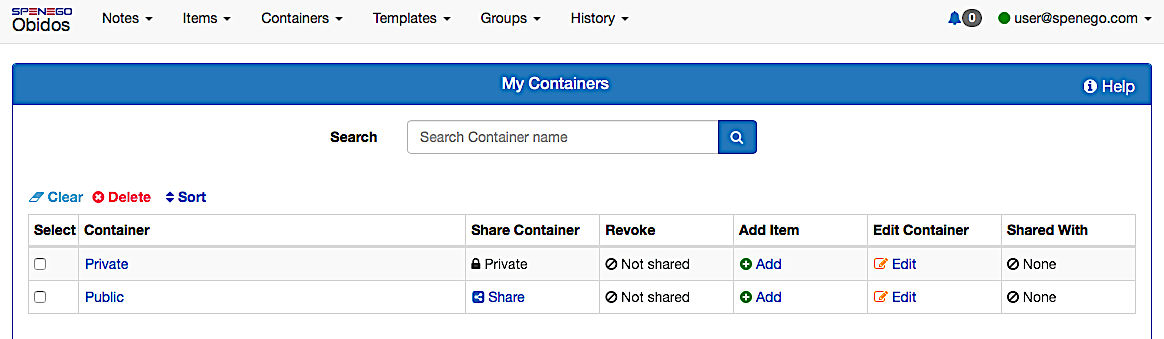
\includegraphics[width=180mm]{user/List-Containers.png}}
\caption{List of Containers}
\label{fig: Figure}
\end{figure}

\section{Delete a Container}

Select "My Containers" from the Container tab. A Container can be deleted only from this list.
Select the Container(s) to delete by clicking on the button to the left of the name(s) of the Container(s).
Then using the {\color{red}\faTimesCircle \ Delete} button on the top, the selected Container(s) can be deleted.
When a Container is deleted, all Items in the Container will be deleted. All Items shared from this Container will be revoked.

\begin{figure}[H]
\centering
\fbox{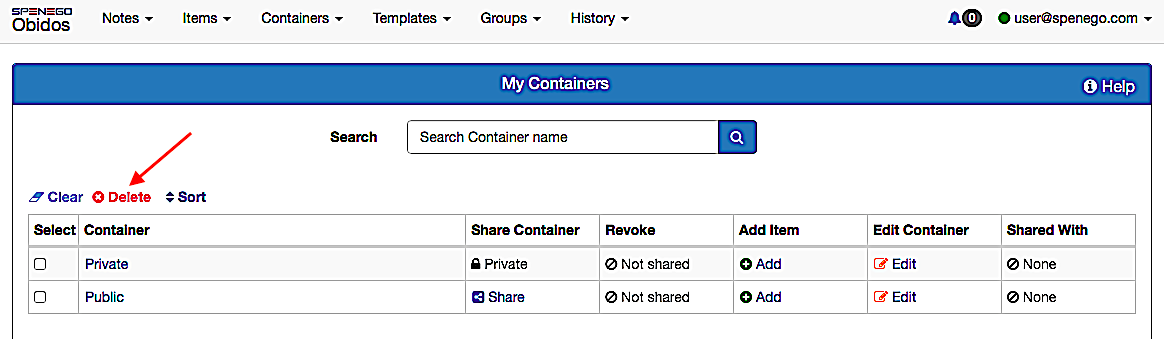
\includegraphics[width=180mm]{user/Delete-Container.png}}
\caption{Delete a Container}
\label{fig: Figure}
\end{figure}

\section{Share Container}
A Container can be shared only if it is of type Shareable.
Sharing a Container is done from "My Containers" list.

\begin{figure}[H]
\centering
\fbox{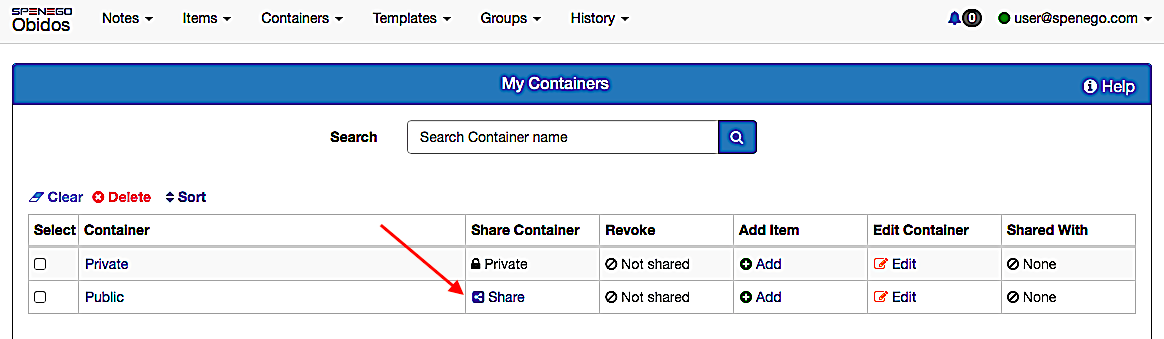
\includegraphics[width=180mm]{user/Share-Container.png}}
\caption{Sharing a Container}
\label{fig: Figure}
\end{figure}

Using the {\color{myblue}\faShareAltSquare \ Share} button on the line corresponding to the Container to be shared,
the sharing process can be initiated.

\section{Changing Name of a Container}
The name of a Container can be changed by editing it.
From "My Containers" list, use {\color{orange}\faEdit} {\color{myblue}Edit} link to initiate the edit process.

\begin{figure}[H]
\centering
\fbox{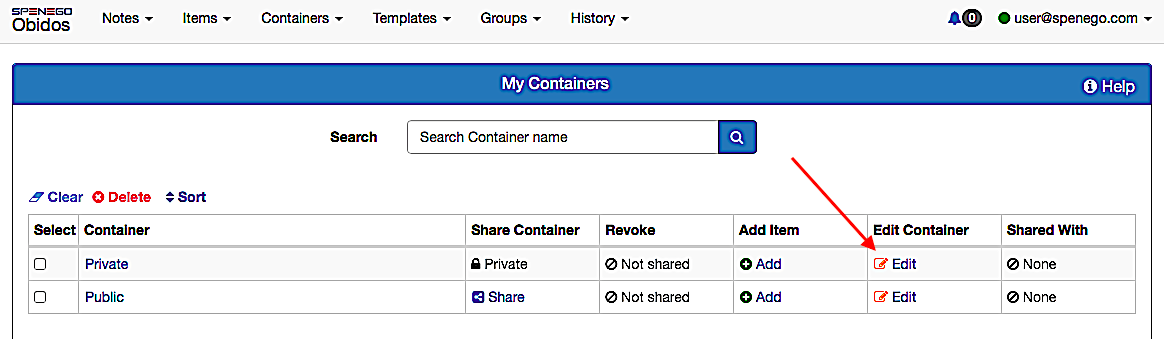
\includegraphics[width=180mm]{user/Edit-Container.png}}
\caption{Edit a Container}
\label{fig: Figure}
\end{figure}

On clicking {\color{orange}\faEdit} {\color{myblue}Edit} link, the screen to edit the Container will appear. 
There you will be able to change the name of the Container.

   \chapter{Items}

Items can be Private or Shareable.
Since an Item has to belong to a Container, the Container must exist or be created first.
A Private Item can be stored in a Private or Shareable Container.
Such an Item cannot be shared with any user.
A Shareable Item can be stored only inside a Shareable Container.

\section{Create an Item}
From Main Menu bar, select "Items" tab and then select "Create new Item".
The screen with the list of Containers will show up.
To create an Item in a specific Container of interest, click on {\color{mygreen}\faPlusCircle} {\color{myblue}Add} link
on the corresponding line. You could also open the Container of interest and then click on 
{\color{mygreen}\faPlusCircle} {\color{myblue}Add} link to add an Item.

\begin{figure}[H]
\centering
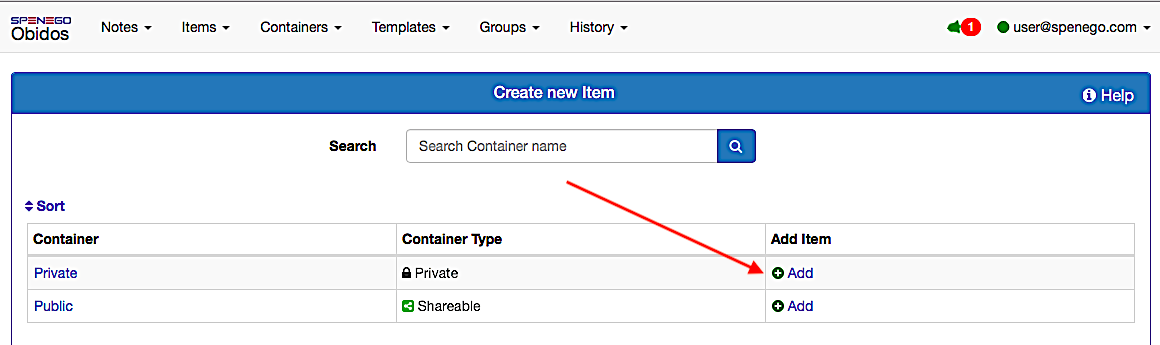
\includegraphics[width=150mm]{user/Items-Add.png}
\caption{Add an Item to a Container}
\label{fig: Figure}
\end{figure}

In the next screen it will be asked to select the type of Item. 

\begin{figure}[H]
\centering
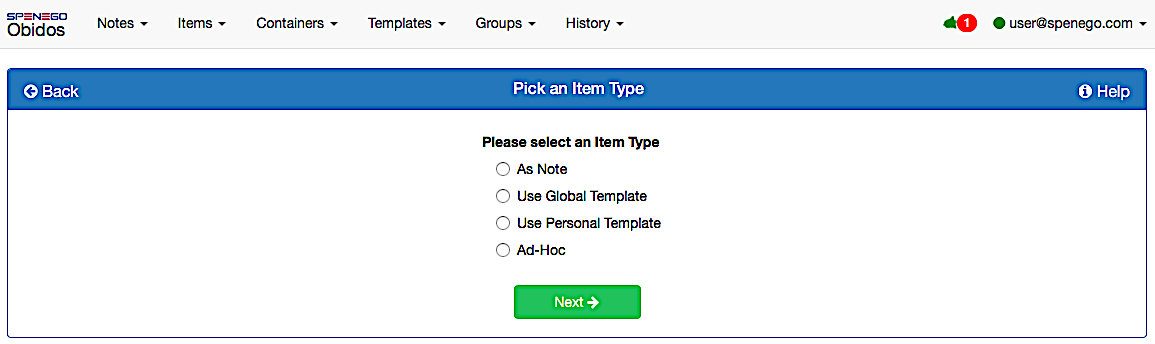
\includegraphics[width=150mm]{user/Item-Type.png}
\caption{Select the Type of the Item}
\label{fig: Figure}
\end{figure}

The Item can be created using a Global Template or Personal Template.
Or the Item can be created as a Note. It is also possible to create an ad hoc Item. An ad hoc item is a free form.
When creating a Shareable Item, it is possible to set an expiration. The user can specify the number of days after which the Item will expire. Once an Item expires, it will not be accessible.
It is not possible to set expiration on a Private Item.

\section{List Items}
Select "Items" from the Main Menu bar and then select "My Items" to set the list of all Items. Each Item will also show the Container
to which it belongs.

\begin{figure}[H]
\centering
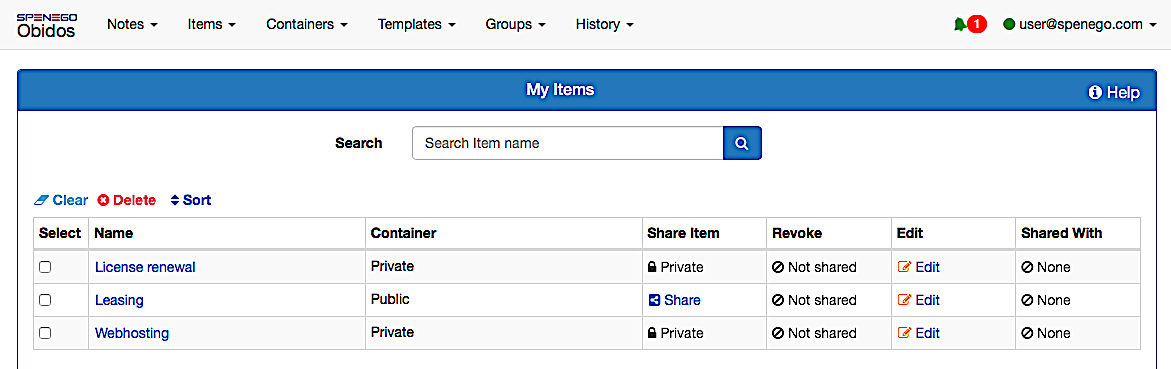
\includegraphics[width=150mm]{user/Items-List.png}
\caption{List Items in a Container}
\label{fig: Figure}
\end{figure}

%\subsection{Sorting the List of Items}
The List of Items can be sorted in alphabetical order either based on Item names or based on Container names.

\begin{figure}[H]
\centering
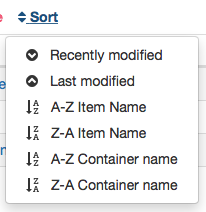
\includegraphics[scale=0.5]{user/Items-Sort.png}
\caption{Sorting Items List}
\label{fig: Figure}
\end{figure}

\section{View an Item}
Get the List of Items (see section above).
From the List of Items, on the line corresponding to the Item, click on the name of the Item of interest

\section{Edit an Item}
Get the List of Items (see section above).
From the List of Items, on the line corresponding to the Item, there will be a button to edit the Item.

\begin{figure}[H]
\centering
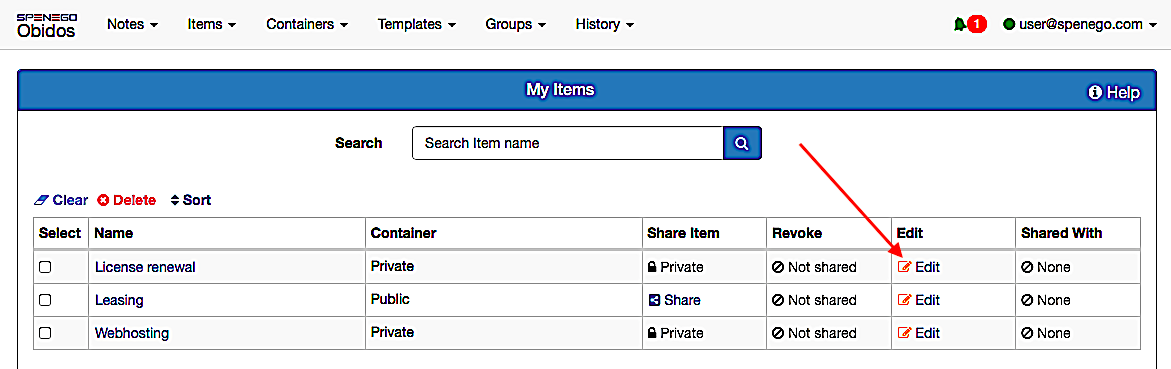
\includegraphics[width=150mm]{user/Items-Edit.png}
\caption{Edit an Item}
\label{fig: Figure}
\end{figure}

\section{Delete an Item}
Get the List of Items (see section above).
From the List of Items, select the Item(s) to delete by clicking on the button on the left of the Item(s). 
Then click on on {\color{red}\faTimesCircle \ Delete} button.

\begin{figure}[H]
\centering
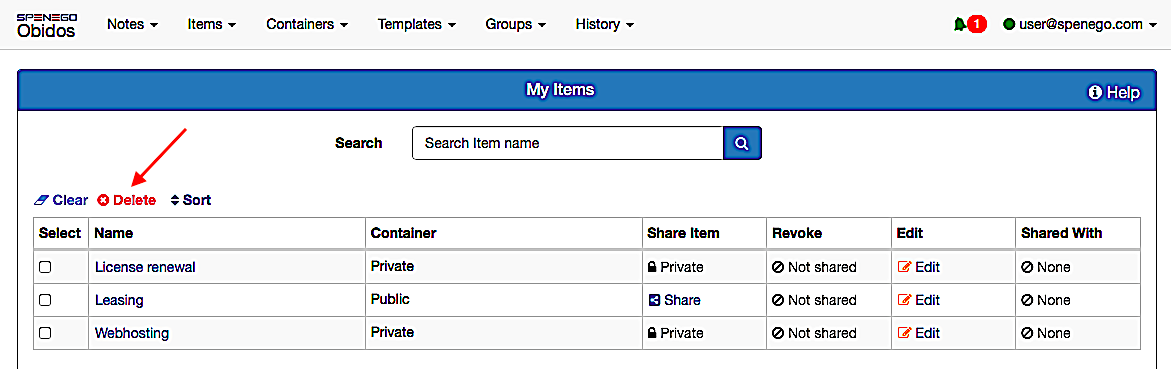
\includegraphics[width=150mm]{user/Items-Delete.png}
\caption{Deleting an Item}
\label{fig: Figure}
\end{figure}

When an Item is deleted, it will be revoked from all users to whom it was previously shared.

\section{Share an Item}
Sharing an Item can be done only from the List of Items (see section above).
From the List of Items, on the line corresponding to the Item, click on {\color{myblue}\faShareAltSquare \ Share} link
to initiate sharing of the Item.

\begin{figure}[H]
\centering
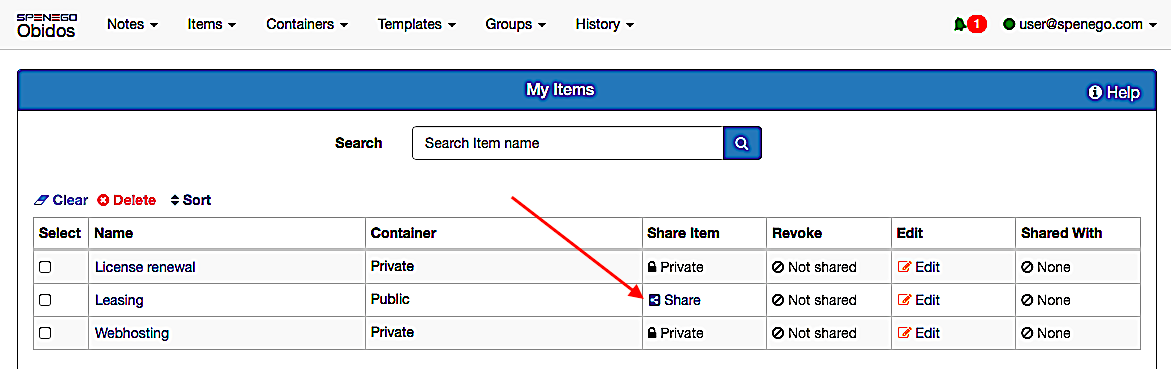
\includegraphics[width=150mm]{user/Items-Share.png}
\caption{Sharing an Item}
\label{fig: Figure}
\end{figure}


   \chapter{Templates}

Regular users can create/modify Personal Templates.
However, the Administrator has to grant special permissions for a regular user to create/modify Global Templates.

\section{Global Templates}
Obidos comes with a number of predefined Global Templates. These Global Templates are available to all users.

\section{Personal Templates}
A Personal Template belongs to an individual user and not available/visible to other users.
A user can create a Personal Template from scratch or create one by cloning a Global Template.

\section{Templates Management}
Other than the visibility, Creation/Modification of Global Templates and Personal Templates are done the same way.
\subsection{Creating a Template}

To create a new Personal Template, select "Create new Personal Template" from the top level Templates menu on the Main Menu bar (see the following Figure).

\begin{figure}[H]
\centering
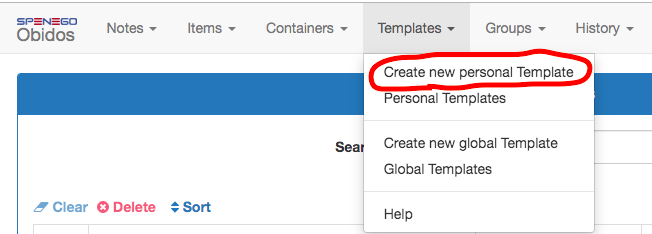
\includegraphics[scale=0.4]{user/Create-Personal-Template-Menu.png}
\caption{Create new Personal Template}
\label{fig: Figure}
\end{figure}

The following figure shows the screen for creation of the Personal Template.

\begin{figure}[H]
\centering
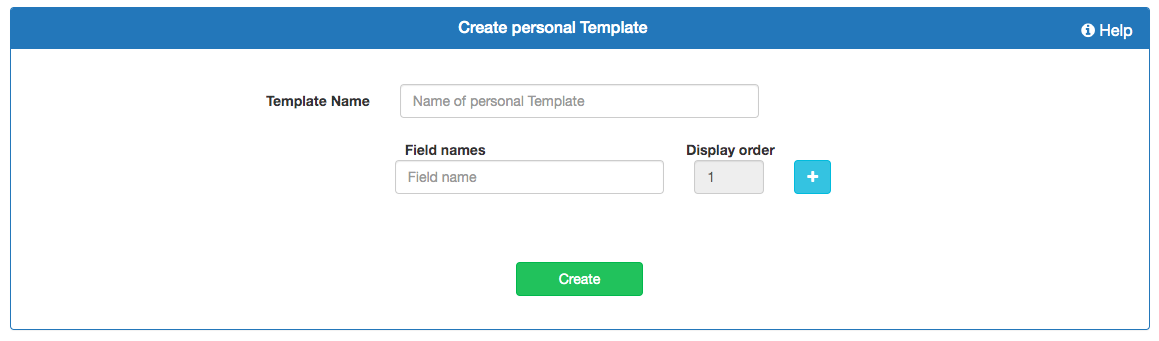
\includegraphics[scale=0.4]{user/Create-Personal-Template-Screen-1.png}
\caption{Screen for new Personal Template}
\label{fig: Figure}
\end{figure}

The name of the Template is used in the listings and searches. It can be upto 64 characters long.
A field name can be upto 32 characters long. The "Display order" decides the order in which the fields
will be displayed from top to bottom. To add a new field, click on the 
{\color{myblue}\faPlusSquare} button. Adding a second field will display a screen as shown in the following Figure.

\begin{figure}[H]
\centering
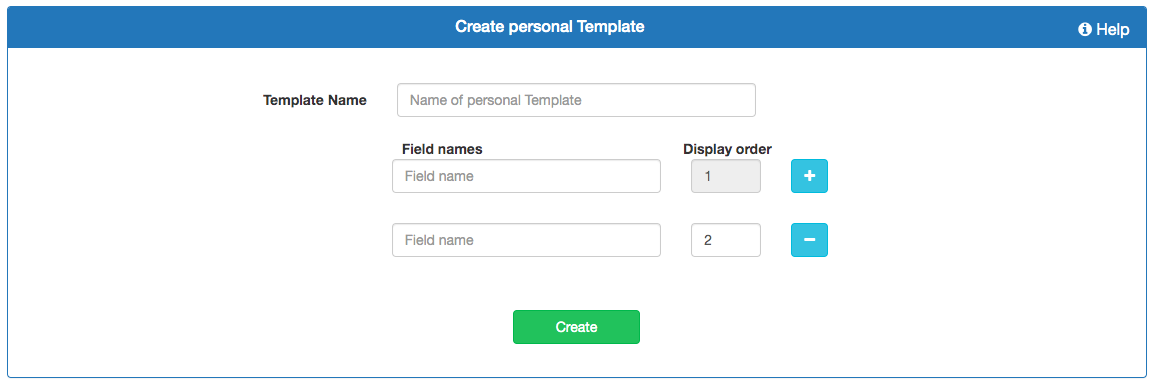
\includegraphics[scale=0.4]{user/Create-Personal-Template-Screen-2.png}
\caption{Adding fields to a Template}
\label{fig: Figure}
\end{figure}

To remove a field, click on the {\color{myblue}\faMinusSquare} button.

\subsection{Creating an Item Using a Template}
Consider a Template named testTemplate with 5 fields as seen in the following Figure.

\begin{figure}[H]
\centering
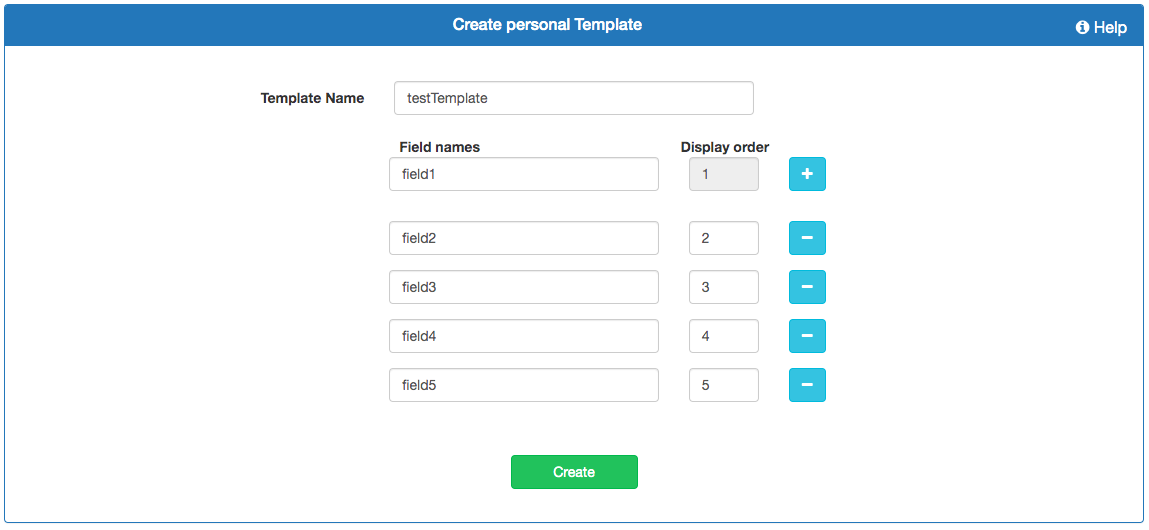
\includegraphics[scale=0.4]{user/Personal-Template.png}
\caption{Personal Template with 5 fields}
\label{fig: Figure}
\end{figure}

When testTemplate is used to create an Item, the screen will present like this:

\begin{figure}[H]
\centering
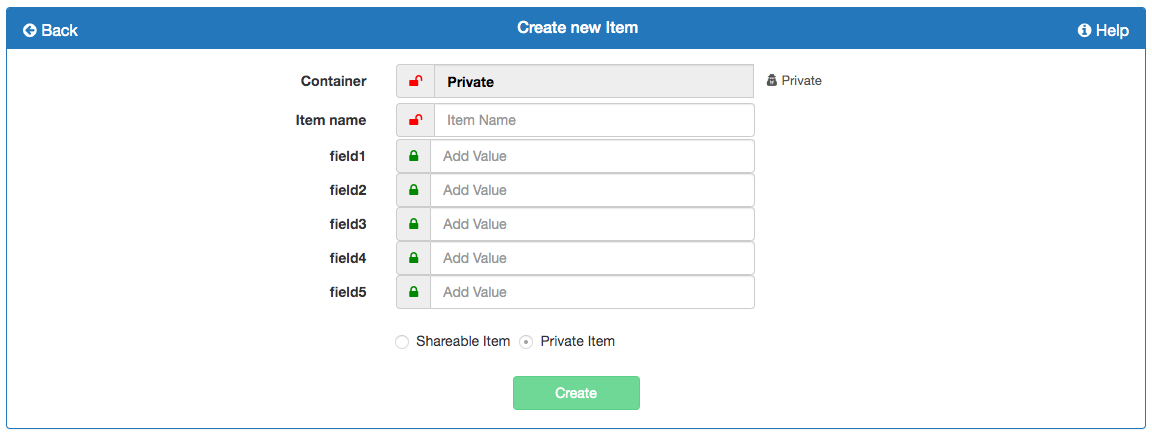
\includegraphics[scale=0.4]{user/Create-Item-With-Personal-Template.png}
\caption{Creating an Item using testTemplate}
\label{fig: Figure}
\end{figure}


   \chapter{Groups}

Any user can create/modify a Group of users. A Group is a set of users identified by a name tag.
A Group belong to an individual user (who is the owner of the Group) and not visible to others.
If sharing is done frequently with a specific set of users, it is probably helpful to create a Group for 
those users. This will make it easy to share with the Group once instead of sharing separately with each of the 
individual users.

\section{Creating a Group}

\begin{figure}[H]
\centering
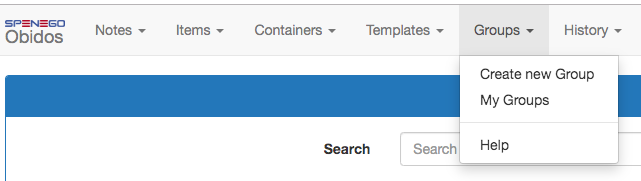
\includegraphics[scale=0.4]{user/Create-Group-Menu.png}
\caption{Creating a Group}
\label{fig: Figure}
\end{figure}

\begin{figure}[H]
\centering
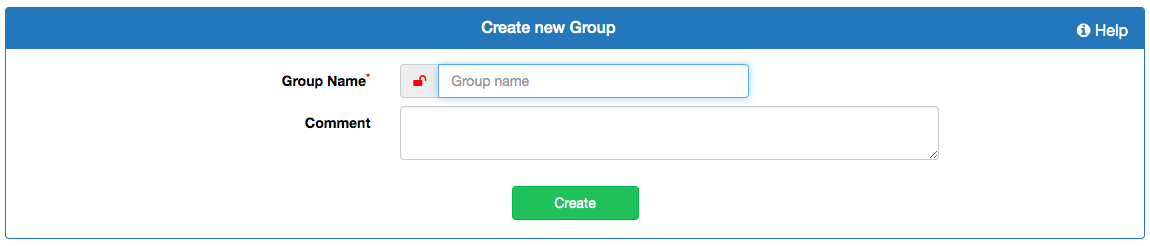
\includegraphics[scale=0.4]{user/Create-Group.png}
\caption{Creating a Group}
\label{fig: Figure}
\end{figure}

\section{Adding Users to a Group}

\begin{figure}[H]
\centering
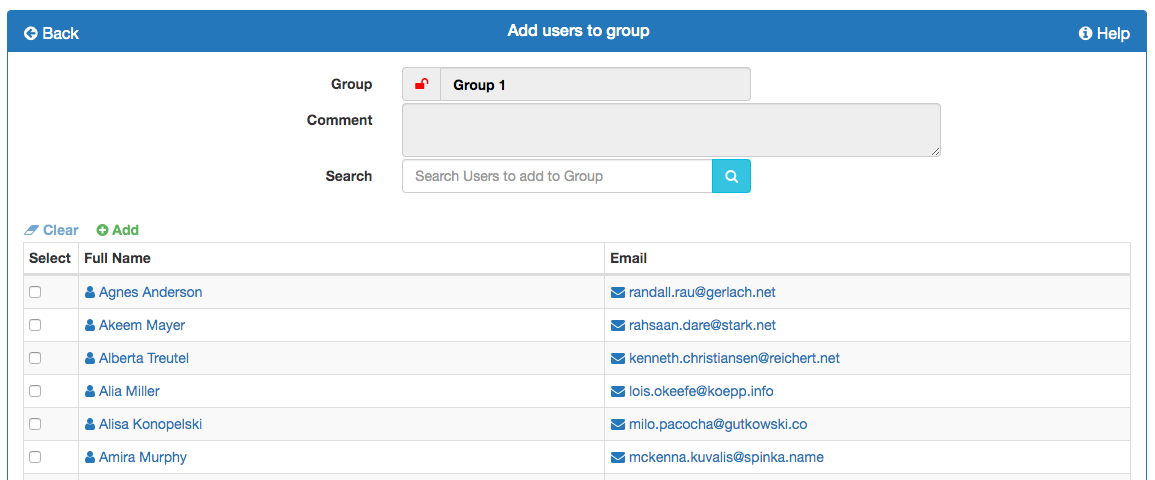
\includegraphics[scale=0.4]{user/Add-Users-to-Group.png}
\caption{Add Users to a Group}
\label{fig: Figure}
\end{figure}

\section{Deleting Users From a Group}

\begin{figure}[H]
\centering
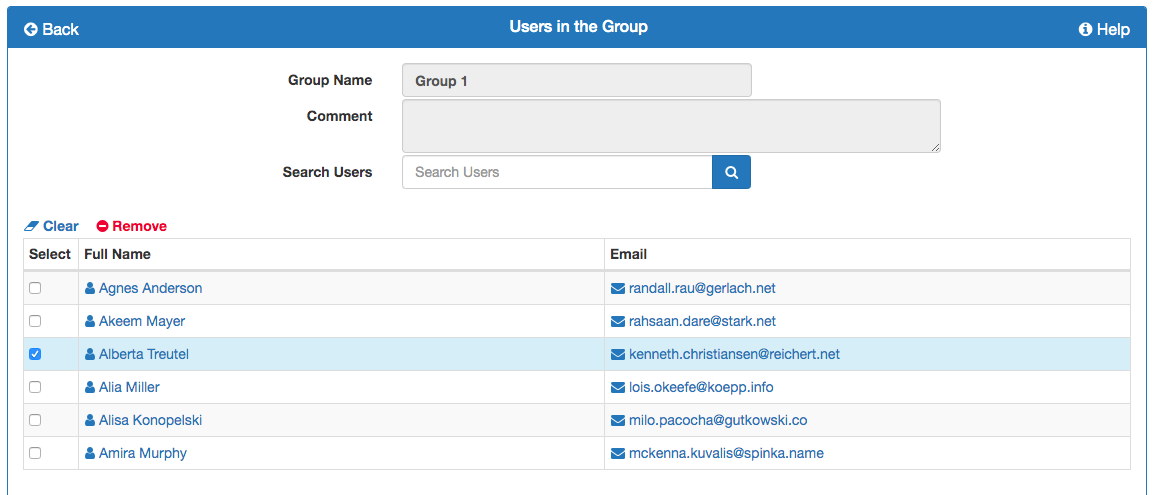
\includegraphics[scale=0.4]{user/Delete-Users-from-Group.png}
\caption{Listing Groups}
\label{fig: Figure}
\end{figure}

\section{Changing Group name}

\begin{figure}[H]
\centering
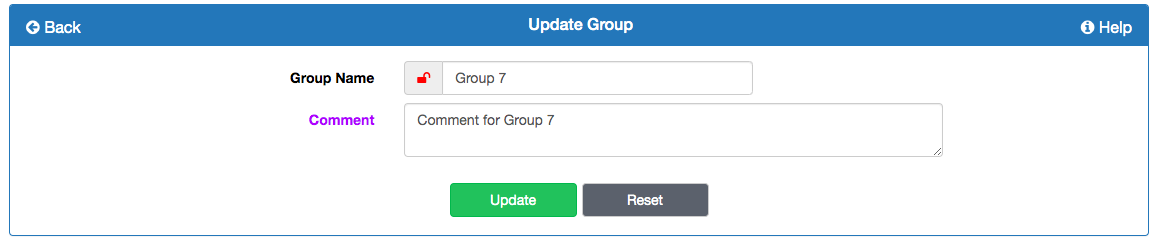
\includegraphics[scale=0.4]{user/Change-Group-Name.png}
\caption{Changing a Group Name}
\label{fig: Figure}
\end{figure}

\section{Listing Groups}

\begin{figure}[H]
\centering
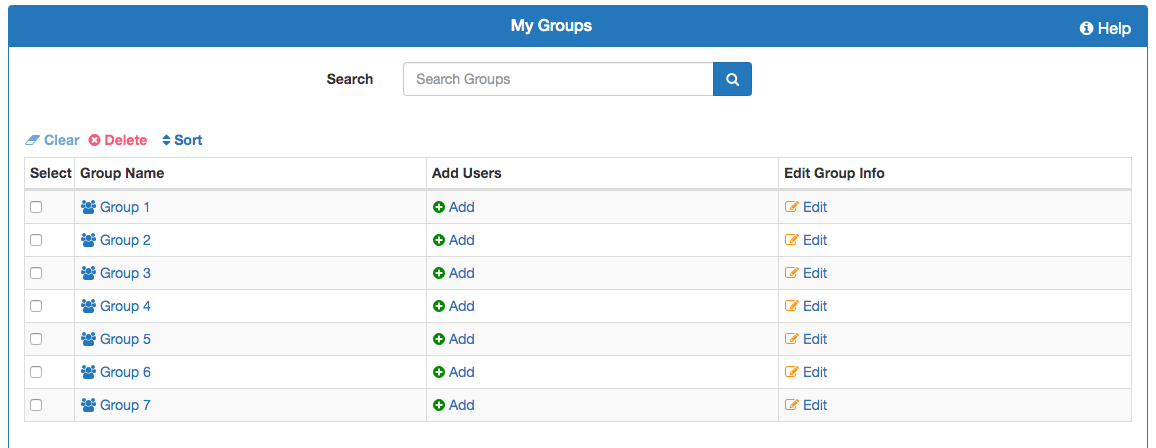
\includegraphics[scale=0.4]{user/Listing-Groups.png}
\caption{Listing Groups}
\label{fig: Figure}
\end{figure}


   \chapter{Activity History}

Obidos shows the history of individual user activities.
This is available in the History menu.

\section{Viewing Activity History}
From the top "History" menu, select "Activity History" (see following figure).

\begin{figure}[H]
\centering
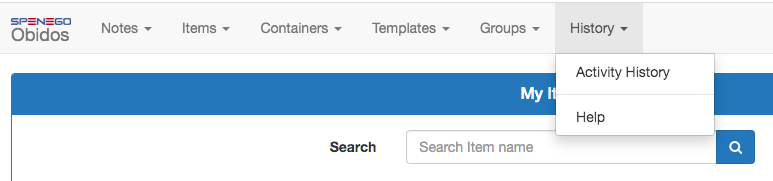
\includegraphics[width=90mm]{user/History-Menu.png}
\caption{Activity History Menu}
\label{fig: Figure}
\end{figure}

The list of activities will be displayed.
There is option to search for history between certain dates/times.
It is also possible to search for activities related to Items/Notes/Containers of interest.

   \begin{appendices}
       \appendixpage
\addappheadtotoc

\pagestyle{plain}
\chapter{Authenticators}

This chapter describes setting up an authenticator app for Two Factor Authentication (2FA) to be used with Obidos.
2FA makes it harder for someone to maliciously change a user's passphrase or local password.
Since changing the passphrase can destroy existing entities created by the User, it is very important to make sure
the authenticity of the User in such a point-of-no-return situation. 2FA essentially gives an extra level of verification.
\newline
\tab Either Google Authenticator or Authy can be used with Obidos. 
Both these apps are available from Google Play for Androids and from iTunes for iPhones.
Google Authenticator is very simple and easy to use. Once set up, it can work even when there is no Internet connection.
Authy is a bit more sophisticated. To configure Authy you need a cell\# and an email address.
If you lose your phone, you can set up Authy on the desktop using the same cell\# and email. That way the configuration
set up for Obidos can be salvaged in case the phone is lost. This is because Authy allows backing up to cloud.
In the following sections we give an outline of setting up both these apps.

\section{Google Authenticator}
Once logged into iTunes, if a search for 'Google Authenticator' will show a screen similar to the following.
The app can be download by clicking on the 'OPEN' button. 

\begin{figure}[H]
\centering
\fbox{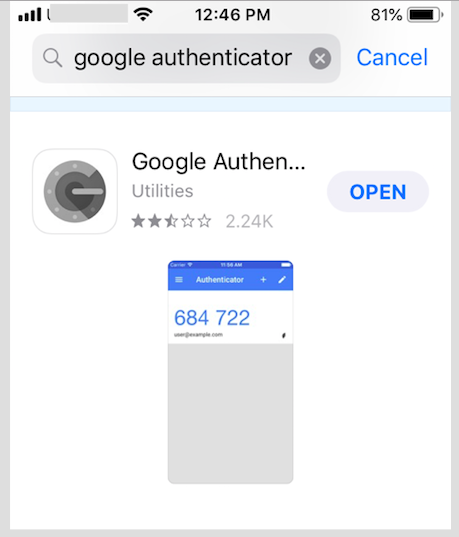
\includegraphics[scale=0.35]{user/Google-Auth-iTunes.png}}
\caption{Google Authenticator in iTunes}
\label{fig: Figure}
\end{figure}

After installing, when opening Google Authenticator, the very first screen will look similar to the 
following figure. Click on 'BEGIN SETUP'.

\begin{figure}[H]
\centering
\fbox{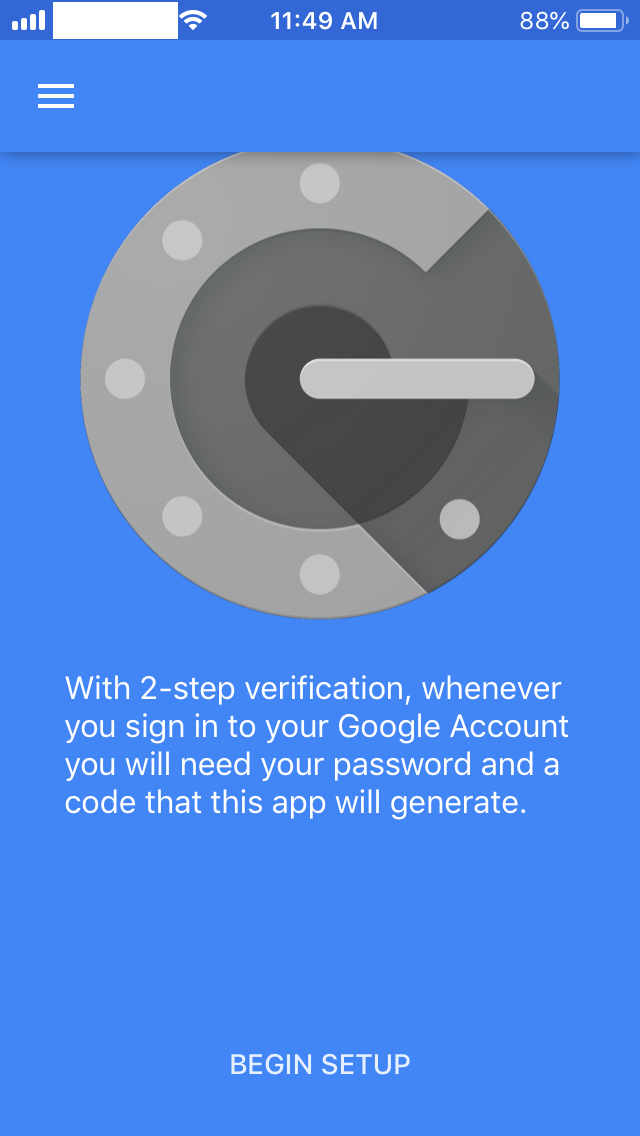
\includegraphics[scale=0.2]{user/Goog-Auth-1.png}}
\caption{Google Authenticator Initial screen}
\label{fig: Figure}
\end{figure}

During setup, there are two options. One is to scan a QR code and the other is to manually
enter the code from Obidos.

\begin{figure}[H]
\centering
\fbox{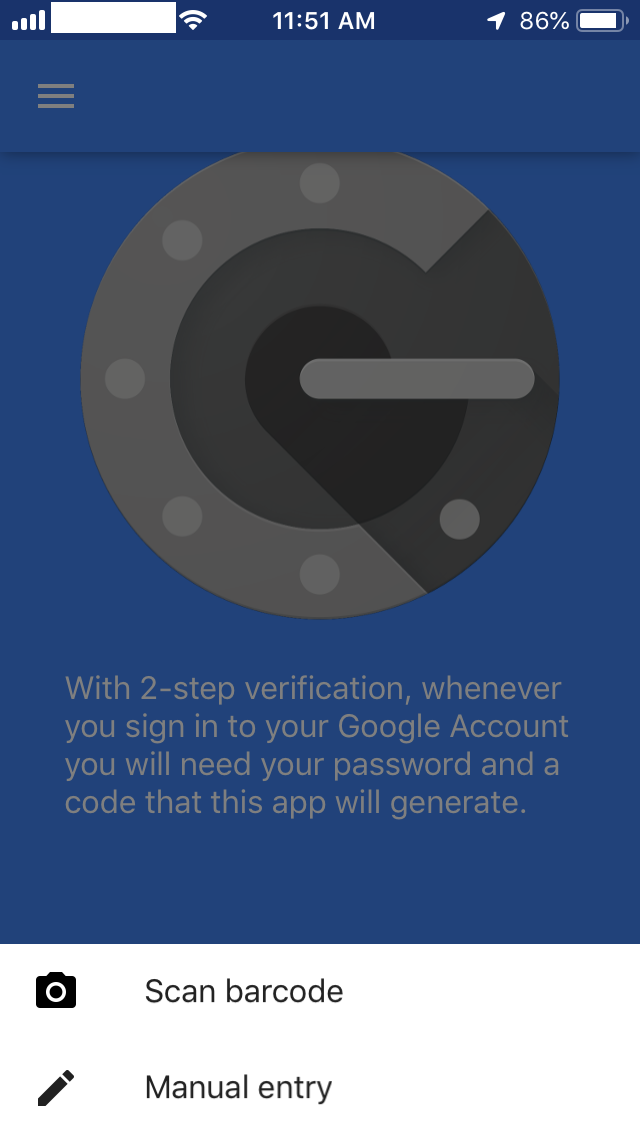
\includegraphics[scale=0.2]{user/Goog-Auth-2.png}}
\caption{Screen to choose between Scanning QR code or entering code manually}
\label{fig: Figure}
\end{figure}

Obidos displays both QR code and the text code. So either the QR code from Obidos can be scanned or
the text code can be manually entered. When the option to scan QR code is selected, the camera will come into focus.
The phone position must be adjusted so that the QR code comes within the green square.

\begin{figure}[H]
\centering
\fbox{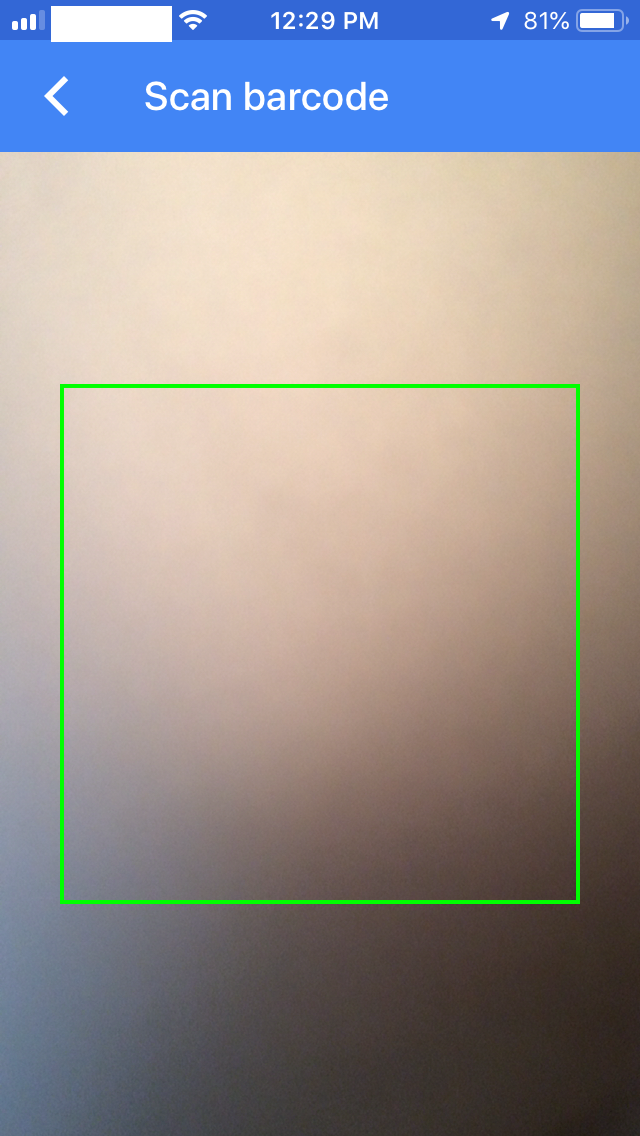
\includegraphics[scale=0.2]{user/Goog-Auth-3.png}}
\caption{QR Code Scanning Frame}
\label{fig: Figure}
\end{figure}

After scanning the QR code from Obidos (or manually entering the code), the Authenticator screen 
will look as in the following figure. 
A six digit code will be displayed and this code will change every 30 seconds.
This is the code that is requited by Obidos whenever 2FA authentication is used.

\begin{figure}[H]
\centering
\fbox{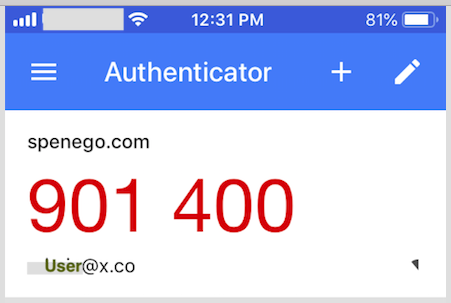
\includegraphics[scale=0.4]{user/Goog-Auth-4.png}}
\caption{Google Authenticator 6 digit code}
\label{fig: Figure}
\end{figure}

\pagebreak

\section{Authy}
In iTunes, searching for 'Authy' will show a screen similar to the following.
Download Authy by clicking on the 'OPEN' button. 

\begin{figure}[H]
\centering
\fbox{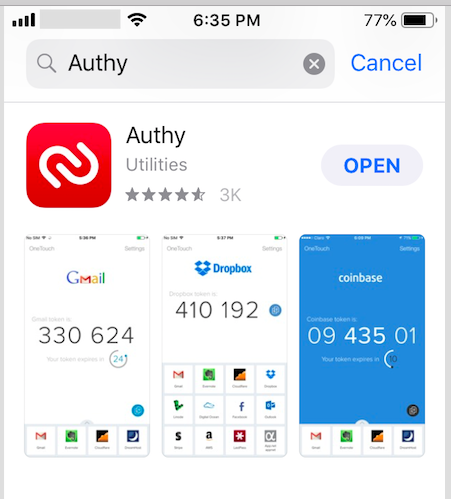
\includegraphics[scale=0.3]{user/Authy-iTunes.png}}
\caption{Authy in iTunes}
\label{fig: Figure}
\end{figure}

When 'Authy' is initially opened, the setup screen will start configuration by asking for cell phone number.
Once the phone number is entered, an email address will need to be provided.

\begin{figure}[H]
\centering
\fbox{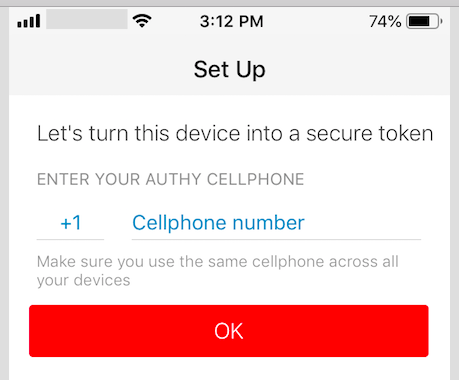
\includegraphics[scale=0.3]{user/Authy-1.png}}
\caption{Authy setup screen}
\label{fig: Figure}
\end{figure}

After entering initial information, Authy will provide you a confirmation code via phone call
or via SMS text. User will be given the choice.

\begin{figure}[H]
\centering
\fbox{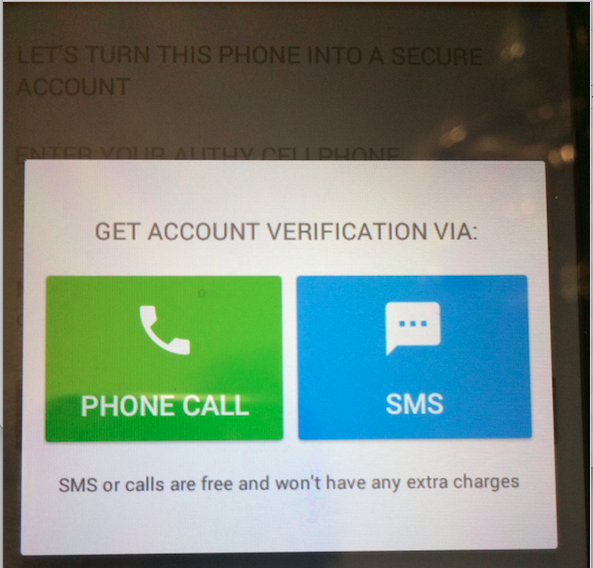
\includegraphics[scale=0.35]{user/Authy-2.png}}
\caption{Mode of communicating confirmation code}
\label{fig: Figure}
\end{figure}

After dispatching the code, Authy will ask the User to enter the confirmation code.

\begin{figure}[H]
\centering
\fbox{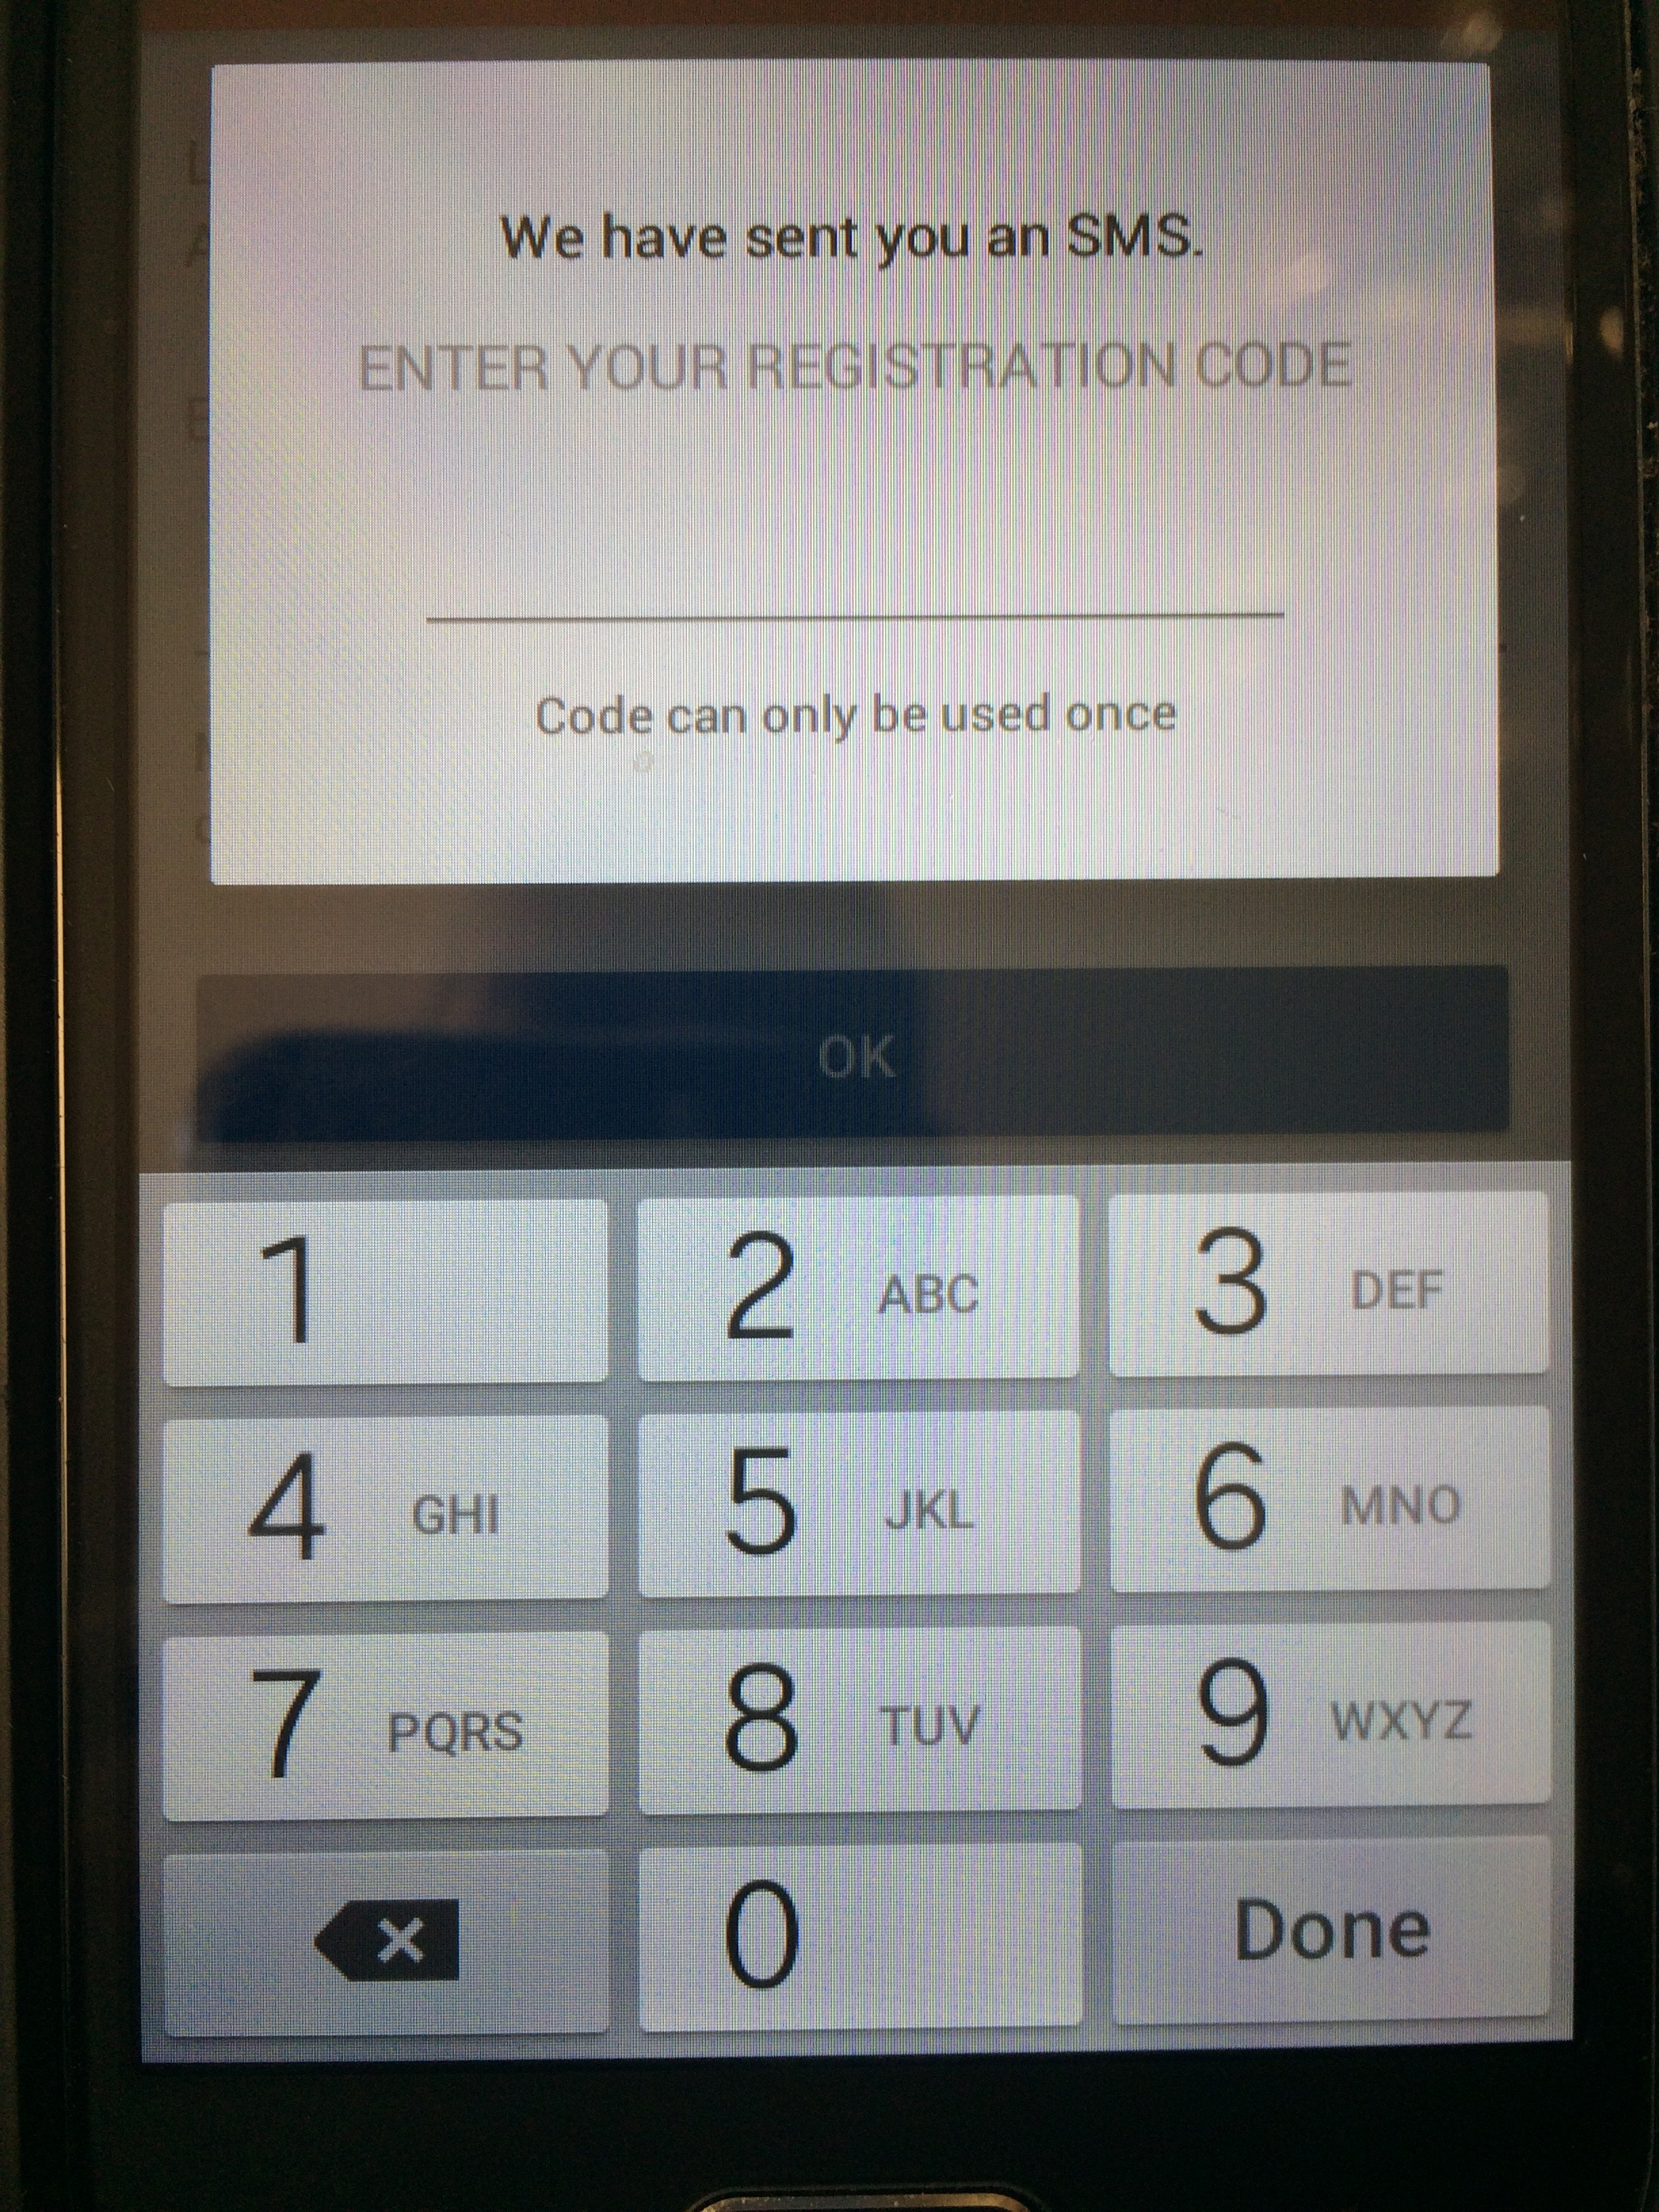
\includegraphics[scale=0.08]{user/Authy-3.jpg}}
\caption{Screen for entering the confirmation code}
\label{fig: Figure}
\end{figure}

Once the confirmation code is validated, it is ready to set up authenticator accounts.

\begin{figure}[H]
\centering
\fbox{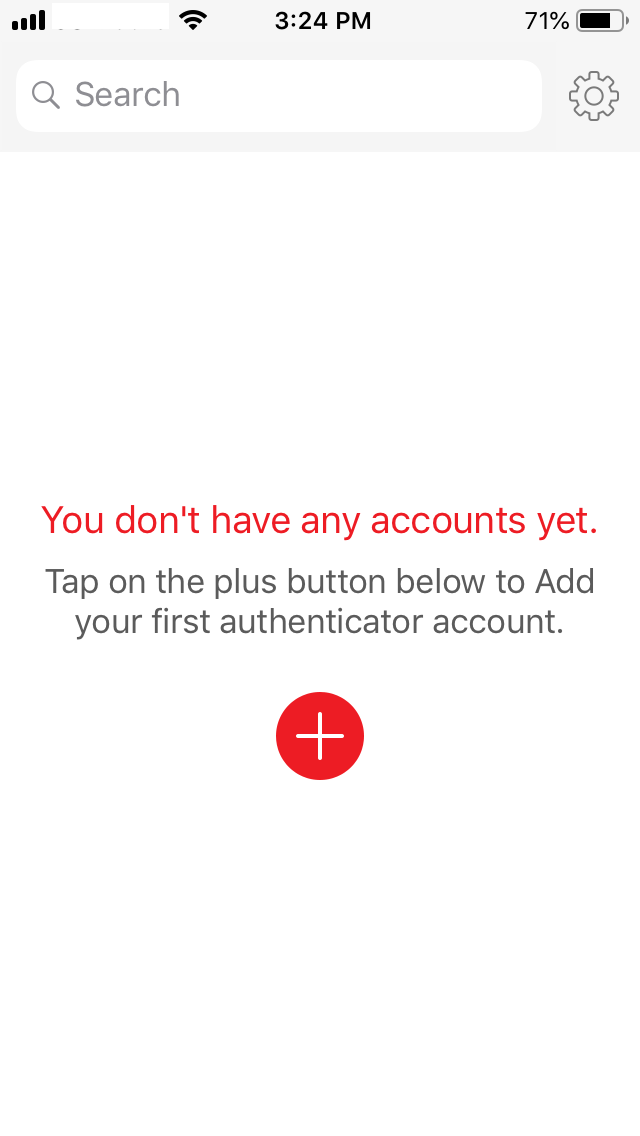
\includegraphics[scale=0.2]{user/Authy-4.png}}
\caption{Ready to set up authenticator accounts}
\label{fig: Figure}
\end{figure}

Press the + button to get started. Now the option to scan a QR code or manually enter a code is seen.

\begin{figure}[H]
\centering
\fbox{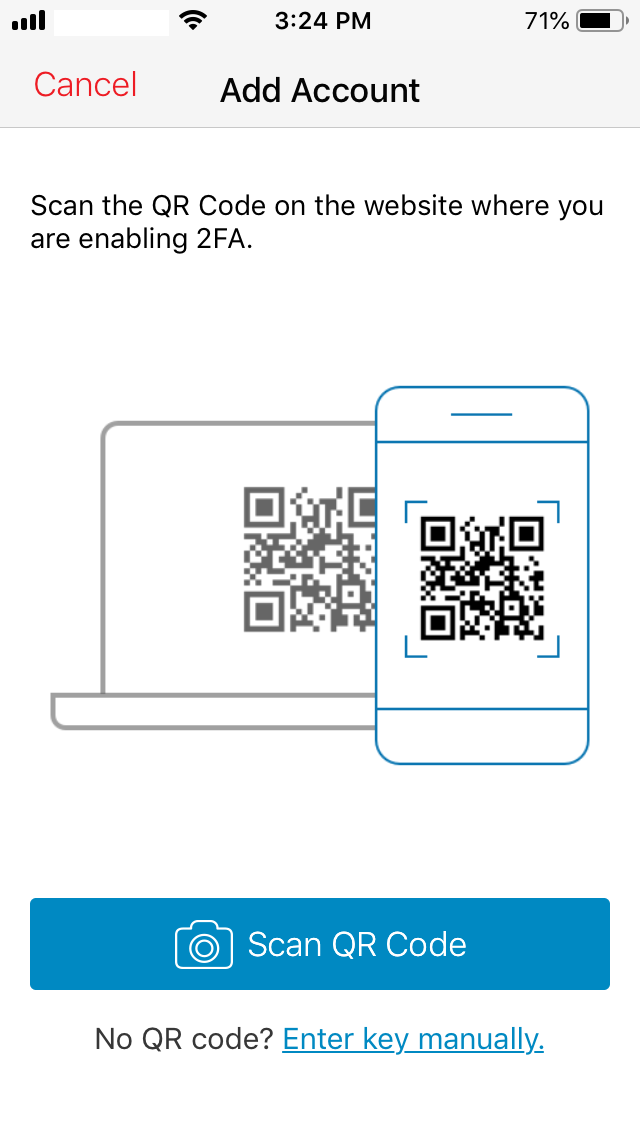
\includegraphics[scale=0.22]{user/Authy-5.png}}
\caption{Enter code from Obidos}
\label{fig: Figure}
\end{figure}

When the code is entered (or scanned in), Authy gives you the option to save your configurations in the cloud.

\begin{figure}[H]
\centering
\fbox{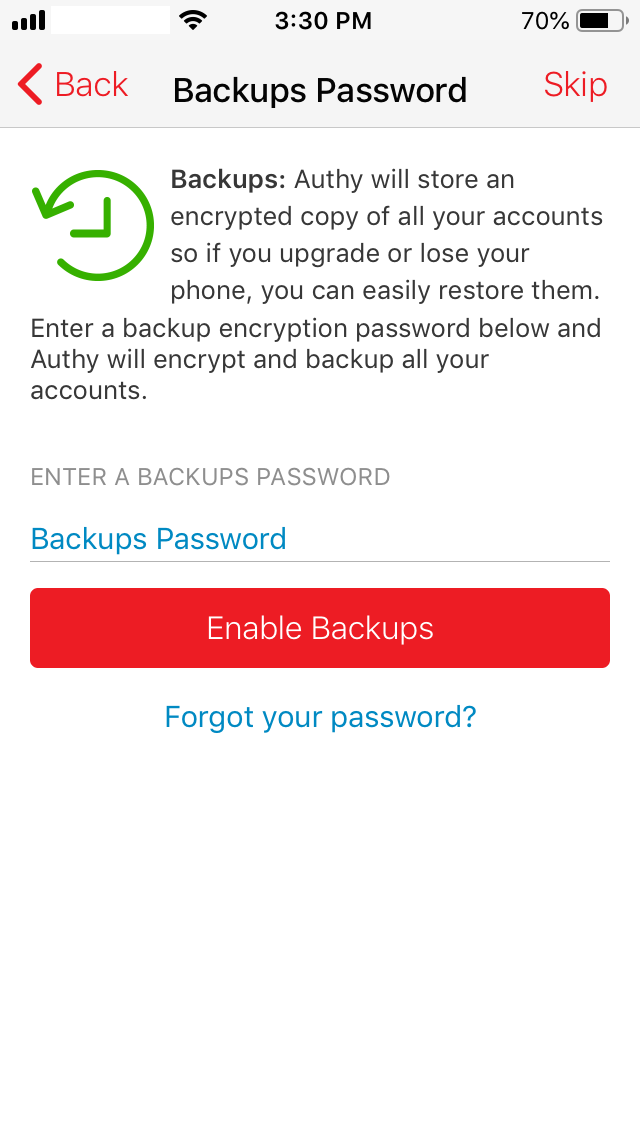
\includegraphics[scale=0.22]{user/Authy-6.png}}
\caption{Cloud backup option}
\label{fig: Figure}
\end{figure}

And finally the scanned code information is presented.

\begin{figure}[H]
\centering
\fbox{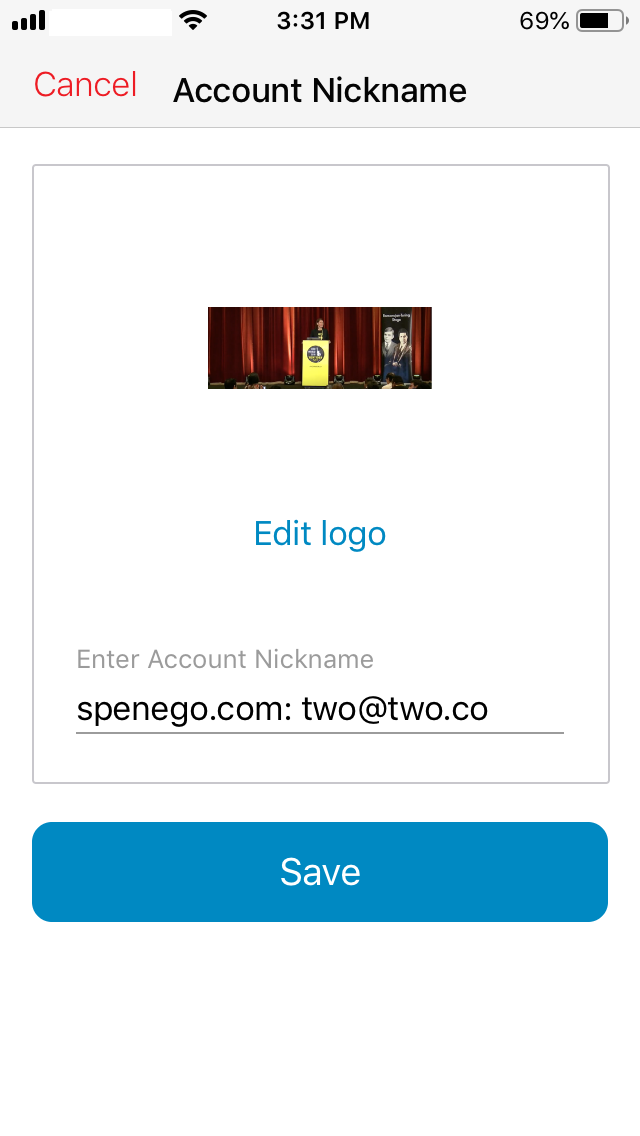
\includegraphics[scale=0.2]{user/Authy-7.png}}
\caption{Save the settings}
\label{fig: Figure}
\end{figure}

Once you save the information, the 6 digt code is displayed. This is the code that Obidos requires when 2FA is used.

\begin{figure}[H]
\centering
\fbox{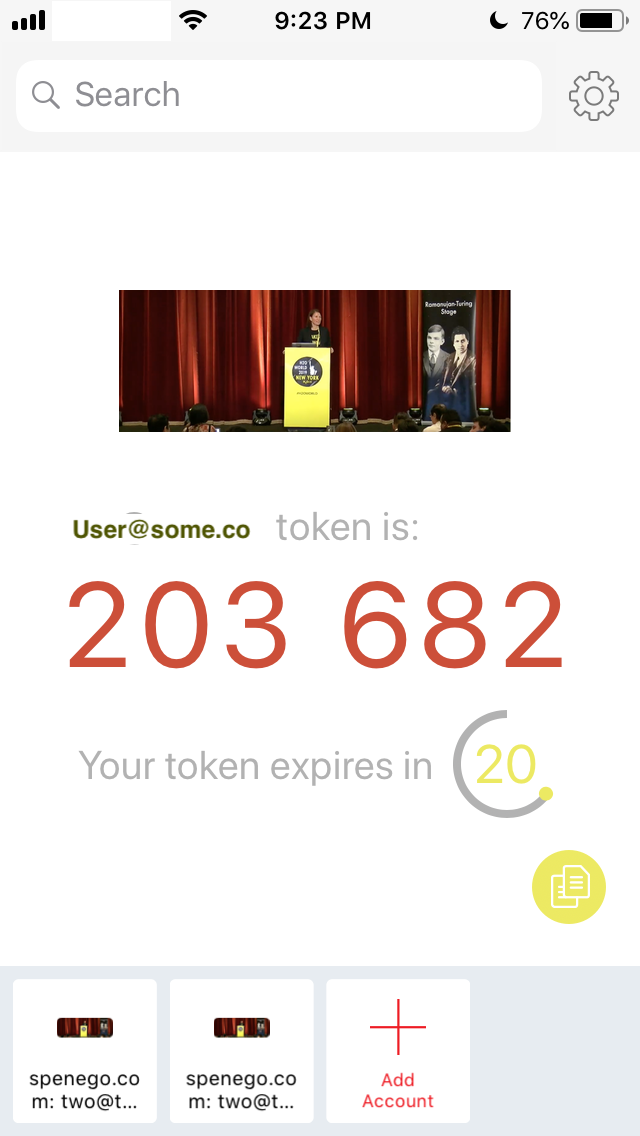
\includegraphics[scale=0.2]{user/Authy-8.png}}
\caption{Authy 6 digit code display}
\label{fig: Figure}
\end{figure}

   \end{appendices}

    % -------------------------------------------------------------------------------------
    % REFERENCES
    % -------------------------------------------------------------------------------------
    %\bibliography{}
    
    % -------------------------------------------------------------------------------------
    % END DOCUMENT
    % -------------------------------------------------------------------------------------
    \end{document}
